% =========================================================================
% AI-Assisted Aircraft Conceptualization:
% Preliminary Design of a Tail-Sitter UAV
%
% Build:  latexmk -pdf main.tex     (or: pdflatex + bibtex + pdflatex x2)
% =========================================================================
\documentclass[11pt,a4paper]{article}

\usepackage[T1]{fontenc}
\usepackage[utf8]{inputenc}
\usepackage{lmodern}
\usepackage[margin=2.5cm]{geometry}
\usepackage{amsmath,amssymb}
\usepackage{graphicx}
\usepackage{booktabs}
\usepackage{multirow}
\usepackage{tabularx}
\usepackage{caption}
\usepackage{subcaption}
\usepackage{rotating}
\usepackage[round,authoryear]{natbib}
\usepackage{tikz}
\usetikzlibrary{arrows.meta,positioning,shapes.geometric,fit}
\usepackage{xcolor}
\usepackage{enumitem}
\usepackage[hidelinks]{hyperref}

% --- editorial helpers (remove before submission) ------------------------
\newcommand{\todopaper}[1]{\textcolor{red}{[TODO: #1]}}
\newcommand{\citeneeded}{\textcolor{red}{[citation needed]}}

% --- shorthand ------------------------------------------------------------
\newcommand{\code}[1]{\texttt{#1}}
\graphicspath{{figures/}}

\title{\textbf{AI-Assisted Aircraft Conceptualization:\\
Preliminary Design of a Tail-Sitter UAV}}

\author{%
  Onur Tuncer$^{1}$
  \and Ahmet G\"une\c{s}$^{2}$
  \and \c{C}a\u{g}lar \"U\c{c}ler$^{3,}$\thanks{Corresponding author:
  \texttt{caglar.ucler@ozyegin.edu.tr}}\\[1ex]
  \small $^{1}$Istanbul Technical University, Faculty of Aeronautics and
  Astronautics, Istanbul, T\"urkiye\\
  \small $^{2}$Istanbul Technical University, Faculty of Naval
  Architecture and Ocean Engineering, Istanbul, T\"urkiye\\
  \small $^{3}$\"Ozye\u{g}in University, Faculty of Aviation and
  Aeronautical Sciences, Istanbul, T\"urkiye%
}
\date{}

\begin{document}
\maketitle

\begin{abstract}
The conceptual design phase fixes most of an aircraft program's key
decisions while information is scarcest, and it remains dominated by
slow, experience-driven, iterative workflows. Existing applications of
artificial intelligence (AI) to aircraft design are fragmented ---
surrogate aerodynamics, isolated optimizers, code assistance --- and no
structured methodology yet integrates AI across the complete conceptual
design process while preserving physics-based rigor. This paper
proposes such a methodology, in which a large-language-model (LLM)
agent acts as an engineering collaborator inside a version-controlled
design repository: every physical model is deterministic, configured,
and under regression test; the AI writes, refactors, and re-converges
those models under natural-language direction from human engineers, and
every design decision is captured as an architecture decision record
with full git-level provenance of AI contribution. Guardrails --- a
machine-readable project constitution, a one-way dataflow pipeline with
typed hand-offs, pinned design-point regression tests, and continuous
integration that re-executes the entire design on every change ---
ensure that the AI accelerates iteration without ever becoming the
source of an engineering number. Alongside the workflow, the paper
contributes an integrative parameter model of electric VTOL UAV
conceptual design --- a classification of every design quantity as a
requirement, free parameter, coupled state variable, derived quantity,
or constraint, a coupling map locating the circular dependencies, the
full set of first-order dimensioning relations, and the constraint
check flow --- which is what makes multidisciplinary change propagation
a checkable operation rather than an act of memory. The methodology is
demonstrated on the
conceptual design of a small electric tail-sitter VTOL UAV (single
ducted fan, jet vanes): starting from mission requirements, the
human--AI team produced a converged, COTS-frozen 2.52\,kg design point
--- thirteen tagged design snapshots, eighteen recorded architecture
decisions, and a sixteen-stage analysis pipeline spanning sizing,
aerodynamics, control authority, vibration, thermal, CAD, and CFD
hand-off --- in under three weeks of part-time work, while independent
expert review remained an integral, documented part of the loop.
Beyond the reduction in development cycle time, the framework raises
the quality of work by removing the dominant error mode of fast-moving
programs --- inconsistent propagation of a design change --- and it
doubles as an instrument for formal design review, since its review
package is regenerated on every run and cannot be stale. The resulting
workflow is aircraft-agnostic and directly transferable to other
rapidly iterating aerospace development programs.
\end{abstract}

\noindent\textbf{Keywords:} artificial intelligence; aircraft
conceptual design; tail-sitter UAV; large language models; agentic
workflows; multidisciplinary design

\section{Introduction}
\label{sec:intro}

\subsection{Research need and gap}

The conceptual design phase establishes the foundation of every
aircraft development program by defining the overall configuration,
mission feasibility, propulsion architecture, structural layout,
subsystem selection, and overall system performance. These early-stage
decisions rely heavily on preliminary sizing calculations, engineering
heuristics, multidisciplinary trade-off analyses, and numerous design
iterations, despite limited available information
\citep{corrado2022,karali2024surrogate}. In recent years, artificial
intelligence (AI) has demonstrated considerable potential in supporting
individual engineering tasks; however, existing applications remain
fragmented and are typically limited to isolated activities such as
surrogate modeling, geometry generation, programming assistance,
optimization, or document preparation
\citep{karali2024mdo,du2026,pliakos2025}. There is still no structured
methodology that systematically integrates AI into the complete
conceptual aircraft design process while preserving physics-based
engineering calculations, multidisciplinary reasoning, and engineering
verification. This need is particularly critical for UAV development,
where rapidly evolving operational requirements, frequent design
updates, and short development cycles demand conceptual design
iterations significantly faster than those traditionally adopted in
conventional aircraft programs \citep{karali2023,shakeri2018}.

A qualitatively new opportunity has emerged with large language model
(LLM) based \emph{agentic} coding tools, which can read, write,
execute, and test an entire engineering codebase under natural-language
direction. Unlike the surrogate-model and optimizer literature, which
replaces expensive physics with learned approximations, an LLM agent
can operate one level higher: it can \emph{build and maintain} the
deterministic physics toolchain itself, propose and implement design
changes across every affected discipline simultaneously, and document
the reasoning --- while the engineering numbers continue to come
exclusively from transparent, testable, physics-based code. How to
harness this capability without sacrificing rigor, traceability, and
verification is, to the authors' knowledge, unaddressed in the aircraft
design literature.

\subsection{Proposed methodology}

This study presents an AI-assisted conceptual aircraft design
methodology that supports the complete early-stage development process
from mission definition to a validated conceptual configuration. The
methodology integrates preliminary aircraft sizing, propulsion sizing,
energy storage estimation, subsystem and equipment selection,
configuration development, structural considerations, and
multidisciplinary engineering evaluations within a unified iterative
framework. Artificial intelligence functions as an engineering
collaborator that accelerates engineering reasoning, alternative
generation, knowledge synthesis, component evaluation, technical
documentation, and design-space exploration, while analytical
calculations remain the basis of all engineering decisions. Numerical
analyses, computational simulations, and external expert findings are
continuously incorporated into successive design iterations, enabling
the conceptual design to evolve through evidence-based refinement
rather than linear development.

The methodology is realized concretely as a \emph{governed
human--AI--repository loop}: the design lives entirely in a
version-controlled repository whose architecture (configuration
$\rightarrow$ physics library $\rightarrow$ notebook pipeline
$\rightarrow$ typed hand-offs $\rightarrow$ CAD/CFD consumers) is
itself part of the method; the AI agent works inside that repository
under a machine-readable set of engineering rules; and every change is
gated by human review, architecture decision records, pinned
design-point regression tests, and continuous integration that
re-executes the full design. To demonstrate applicability, a
tail-sitter VTOL UAV is developed as an illustrative case study,
covering the process from mission requirements to preliminary sizing,
subsystem selection, configuration development, commercial
component freeze, and hand-off to higher-fidelity validation.

The work is guided by the following research question:

\begin{quote}
\textbf{RQ:} \emph{How can AI accelerate conceptual aircraft design
while preserving physics-based engineering rigor?}
\end{quote}

\subsection{Main contributions}

The primary contribution of this work is the introduction of a
structured AI-assisted methodology for conceptual aircraft design that
integrates preliminary engineering calculations, multidisciplinary
subsystem selection, engineering knowledge management, numerical
analyses, and iterative design refinement into a single coherent
workflow. Unlike existing AI applications that support isolated
engineering tasks, the proposed methodology formalizes the interaction
between human engineering expertise, an LLM-based AI agent, analytical
models, and validation activities throughout the conceptual design
process --- including the guardrails (design-point regression pins,
one-way dataflow, decision records, standing-finding discipline) that
make AI acceleration compatible with engineering accountability. The
framework is aircraft-independent and can be adapted to a wide range of
aerospace platforms that require rapid, multidisciplinary conceptual
development.

As a second contribution, the paper presents an \emph{integrative
parameter model} of electric VTOL UAV conceptual design: an explicit
classification of every design quantity into requirements, free
parameters, coupled state variables, derived quantities, and
constraints; a coupling map showing which factors influence which and
where the circular dependencies lie; the complete set of first-order
dimensioning relations that implement it; and the flow of constraint
and verification checks through which each iteration must pass. This is
the part of a heritage design capability that emerging drone
organizations most conspicuously lack, and it is what makes
multidisciplinary change propagation --- by a human or by an agent ---
a checkable operation rather than an act of memory.

As a third contribution, the paper demonstrates the practical
implementation of the methodology through the conceptual design of a
tail-sitter VTOL UAV, resulting in a complete preliminary sizing
procedure, propulsion system selection, onboard equipment architecture,
and configuration development, together with quantitative process
evidence extracted from the project's own git history: the share of
AI-co-authored engineering commits, the cadence of design-point
snapshots, and the mechanisms by which errors were caught. Furthermore,
the tail-sitter case study provides application-specific engineering
insights into the conceptual development of this unconventional
aircraft configuration, illustrating how AI-assisted multidisciplinary
workflows can reduce development effort while maintaining engineering
rigor, traceability, and design quality.

The remainder of the paper is organized as follows.
Section~\ref{sec:related} reviews AI applications in conceptual
aircraft and UAV design and motivates the tail-sitter as a validation
case. Section~\ref{sec:method} presents the methodology.
Section~\ref{sec:model} presents the integrative parameter model, the
dimensioning relations, and the constraint check flow on which the
methodology operates. Section~\ref{sec:results} reports the case study
results and process metrics and discusses them against the research
question. Section~\ref{sec:conclusions} concludes.

\section{AI and Conceptual Design}
\label{sec:related}

This review covers three linked needs: why AI-assisted conceptual
design is needed in aircraft and especially UAV development, which AI
tools and frameworks already exist, and why a tail-sitter VTOL UAV is a
useful validation case relative to other eVTOL architectures.

\subsection{Design need}

Aircraft conceptual design is still constrained by long, costly,
iterative workflows that must reconcile aerodynamics, structures,
propulsion, stability, manufacturing, and mission requirements early,
when most key decisions are fixed
\citep{karali2024surrogate,corrado2022,lukyanov2024}. Conventional
sequential methods depend heavily on designer experience and
low-fidelity semi-empirical models, which are especially weak for UAVs
because many UAV sizes, Reynolds-number regimes, and unconventional
layouts fall outside the historical data behind those regressions
\citep{karali2024surrogate,lukyanov2024}.

UAV design sharpens this need because UAVs can adopt tailless,
blended-wing, morphing, tandem, canard, and other nontraditional
configurations that demand broader design-space exploration and tighter
coupling between mission definition and vehicle architecture
\citep{karali2024surrogate,ivanova2025,lukyanov2024}. High-fidelity CFD
and finite-element analyses improve realism, but thousands of
evaluations across optimization loops make direct early-stage use
computationally prohibitive, motivating automation, surrogates, and
concurrent multidisciplinary design optimization (MDO) workflows
\citep{karali2024surrogate,wang2023,pliakos2025,leng2024}.

\begin{itemize}[nosep]
\item Early MDO detail is needed to reduce late development setbacks
  and resolve the conceptual-stage ``design paradox'' while design
  freedom remains high \citep{corrado2022}.
\item UAV programs need faster iteration because competition, budget
  limits, and expanding mission complexity make broad manual concept
  trades increasingly impractical
  \citep{karali2023,pliakos2025,shakeri2018}.
\item AI is increasingly relevant because modern UAVs already rely on
  autonomy, real-time decision-making, and mission adaptation under
  battery and payload constraints
  \citep{ivanova2025,sai2023,mcenroe2022}.
\end{itemize}

\subsection{AI tools and frameworks}

The literature points to a clear pattern: AI in conceptual aircraft
design is used less as a replacement for physics than as a
computational amplifier around physics-based models, MDO loops, and
design iteration. The dominant tools are surrogate models for
aerodynamics, structural mass, and sometimes radar cross-section;
evolutionary or multiobjective optimizers; automated geometry/CFD
pipelines; and data-mining or multi-fidelity schemes that reduce
coupling and computational burden
\citep{karali2024surrogate,leng2024,pliakos2025}.

Reported frameworks already support configuration selection, early
sizing, and iterative refinement. AI-supported UAV conceptual design
frameworks compare alternative configurations using learned
disciplinary models, feed optimized results back into sizing, and can
cut runtime dramatically; one deep-learning surrogate framework
reported more than three orders of magnitude computational-time
improvement over traditional methods \citep{karali2024surrogate}. The
methodological frontier is widening toward uncertainty-aware MDO,
digital twins, generative AI, and automated data-generation pipelines
that make high-quality training data easier to produce
\citep{karali2024surrogate,wang2023,du2026,pliakos2025}.

Table~\ref{tab:methodclasses} summarizes representative AI-supported
methodology classes reported for aircraft and UAV conceptual design.

\begin{table}[htbp]
\centering
\caption{Representative AI-supported methodology classes reported for
aircraft and UAV conceptual design.}
\label{tab:methodclasses}
\small
\begin{tabularx}{\textwidth}{@{}lXX@{}}
\toprule
\textbf{Method class} & \textbf{What it supports} &
\textbf{Representative evidence} \\
\midrule
ANN / deep surrogates &
Fast aerodynamics, mass, RCS prediction for concept comparison and
sizing &
AI-driven UAV frameworks use learned aerodynamics, structural mass,
and RCS models in early design \citep{karali2024surrogate} \\
\addlinespace
Evolutionary / GA / DE / multiobjective optimization &
Configuration search, wing optimization, takeoff-weight reduction,
trade-space exploration &
GA{+}ANN wing optimization and DE-based UAV optimization are
established \citep{boutemedjet2019,komarov2024} \\
\addlinespace
Multi-fidelity / data mining &
Variable screening, disciplinary decoupling, cheap-to-expensive
optimization progression &
Multi-fidelity data mining uses low-cost data first, then CFD
fine-tuning \citep{leng2024} \\
\addlinespace
Automated CFD pipelines &
Rapid geometry, meshing, solver setup, dataset generation &
Python-based preprocessing reduces turnaround to minutes with
sub-5\% deviation from expert setups \citep{pliakos2025} \\
\addlinespace
Generative / emerging AI &
Parameterization, predictive modeling, training facilitation,
constraint handling &
GenAI applications now span VAE, GAN, diffusion, and transformer
approaches \citep{du2026} \\
\addlinespace
LLM / agentic coding assistants &
Building and maintaining the analysis toolchain itself;
multidisciplinary change propagation; documentation &
This work; general-purpose agentic tools \citep{anthropic2025claudecode} \\
\bottomrule
\end{tabularx}
\end{table}

\begin{itemize}[nosep]
\item Reinforcement learning is widely used in AI-integrated UAV
  systems, while federated and distributed learning frameworks are
  emerging quickly \citep{sai2023}.
\item AI toolchains increasingly include libraries, frameworks, and
  edge/embedded deployment pathways, not just offline design
  optimizers \citep{sai2023,mcenroe2022}.
\item Current gaps remain important: many studies still focus on
  airfoils or wings rather than full-aircraft models, and robust
  treatment of uncertainty, unconventional configurations, and broader
  objective sets is still developing
  \citep{karali2024surrogate,wang2023,lukyanov2024}.
\end{itemize}

Notably, none of the surveyed frameworks employs AI at the
\emph{workflow} level --- as an agent that authors, verifies, and
evolves the design toolchain and its documentation under human
direction. That is the niche addressed by the present methodology.

The workflow of aircraft design is complex by nature, and it requires
the concurrent facilitation of resources. While large organizations are
privileged to draw on heritage knowledge systems --- accumulated
sizing databases, validated in-house tools, and the tacit experience of
long-lived design teams --- emerging aviation organizations lack this
background and these resources, which further complicates the
situation. Furthermore, small- and large-scale drone development is an
emerging field with significant constraints on development time and
resources, in which design teams are frequently integration-driven
rather than analysis-driven. Consequently, drone development
organizations need a workflow-level framework: one that supplies the
missing bookkeeping and verification discipline itself, instead of
assuming it as institutional heritage. Such a framework is illustrated
herewith for the tail-sitter drone concept explained next.

\subsection{Tail-sitters versus eVTOLs}

Tail-sitter VTOL UAVs are a strong validation case because they force a
conceptual design method to address the hardest coupling in VTOL
design: hover, wing-borne cruise, and the transition between them.
Recent VTOL design studies argue that transition and climb are often
oversimplified in conceptual design even though they strongly drive
motor and battery sizing \citep{kaneko2024}. For tail-sitters
specifically, nonlinear dynamics during transition are a central
limitation, with widely varying speed and attitude, unstable
long-period behavior in some regimes, and controller sensitivity to
uncertainty \citep{yang2024}.

That coupling has a two-decade experimental and control heritage.
Early work established integrated dynamic modeling, control design,
and trajectory generation for miniature autonomous tail-sitters
\citep{knoebel2006}, and demonstrated hover, transition, and level
flight with mode-dependent control laws on a single-propeller indoor
platform \citep{frank2007} --- the same control-architecture problem
the present single-propulsor vehicle poses. Transitional flight of a
small tail-sitter was analyzed at the conceptual level early on
\citep{kubo2008}, and the T-wing program demonstrated autonomous
vertical takeoff, transition, wing-borne flight, and landing in
flight test \citep{stone2008}. Subsequent work carried the maneuver
from analysis into practice: comprehensive flight-control design
validated in experiment \citep{jung2013}, optimal control of the
transition phases to manage control inputs and altitude excursion
\citep{banazadeh2016}, and hardware-in-the-loop simulation linking
the dynamic model to autopilot integration \citep{sun2017}.

Against that difficulty, tail-sitters offer a simpler airframe than
many other eVTOL classes. Compared with tilt-rotor or dual-system
eVTOLs, tail-sitter eVTOLs remove tilting mechanisms and redundant
propulsors, which can reduce structural and mechanical complexity
\citep{yang2024}. But that simplicity trades for harder transition
physics: the aircraft must sustain pitch authority through a full
$90^{\circ}$ rotation, propulsors must provide both high vertical
thrust and efficient forward-flight operation, and oblique inflow
during transition can excite propeller vibration \citep{yang2024}.

\begin{itemize}[nosep]
\item Trajectory-coupled optimization materially matters for
  tail-sitters: simultaneous design-and-trajectory optimization reduced
  energy by 29\% versus uncoupled optimization in one tail-sitter
  delivery case \citep{kaneko2024}.
\item Optimized transition control improves operations, with reduced
  transition time and altitude excursion relative to traditional
  linear transition methods \citep{yang2024}.
\item A tail-sitter validation example is methodologically valuable
  because it stress-tests whether an AI-assisted conceptual design
  framework can integrate physics, controls, propulsion, and sizing in
  one loop rather than treating configuration choice and transition
  performance separately \citep{kaneko2024}.
\end{itemize}

Two further strands of the recent AIAA literature bear directly on
the methodological questions of this paper. The first is model
fidelity: comparisons of aerodynamic models for optimizing
tail-sitter takeoff and transition show that the required fidelity
depends on the question asked of the model \citep{anderson2021},
multi-fidelity analysis of the hover-to-cruise transition quantifies
what low-order models miss in the wake-dominated mid-transition
regime \citep{arias2025}, and integrated
modeling--simulation--control studies of small tail-sitter platforms
illustrate the level of longitudinal-dynamics representation such
vehicles ultimately need \citep{pricker2023}. The second is
operational robustness: transition and re-transition can be defined
as robust, repeatable procedures with explicit corridors and margins
rather than as isolated maneuvers \citep{marvakov2021}; robust
control addresses the large aerodynamic-coefficient changes between
hover, transition, and cruise \citep{kumar2024}; systematic
transition strategies for the closely related tilt-wing class
provide a methodological basis for corridor definition
\citep{may2024}; and descent-rate limits against vortex-ring-state
encounters constrain VTOL landing trajectories \citep{jeong2024}.

The single-duct configuration studied here also carries its own
aerodynamic literature. A dedicated transition method exists for
ducted-fan tail-sitter UAVs \citep{zhang2013}, and nondimensional
models of ducted-fan aerodynamics capture the duct--rotor--airframe
interaction in a form that scales across the flight envelope
\citep{ohanian2012}. Hover performance --- duct lift share, inlet
and diffuser effects, rotor loading --- has been characterized
numerically \citep{sheng2015} and experimentally as a function of
duct geometry \citep{dorfling2023}, and the rotor and duct have been
treated as a single coupled, surrogate-assisted optimization problem
\citep{qing2019} --- a direct methodological precedent for
AI-assisted coupled sizing. Installation effects matter as well:
embedding electric ducted fans close to lifting surfaces changes
both fan and airframe behavior \citep{alabdali2025}; wake
impingement on a nearby surface differs between ducted and unducted
propulsors, directly relevant to a tail-sitter that takes off and
lands with its duct axis normal to the ground \citep{kopperstad2025};
and wing--propeller interaction experiments on hybrid VTOL
configurations show that slipstream effects belong in the conceptual
loop \citep{hrishikeshavan2013,hrishikeshavan2014}.

Taken together, the literature supports an AI-assisted conceptual
design methodology that augments physics-based analysis rather than
replacing it, is especially justified for UAVs with unconventional
configurations, and is well validated by a tail-sitter VTOL case
because tail-sitters expose exactly the multidisciplinary and
transition-coupled trade-offs that simpler conceptual methods tend to
miss.

\section{Method}
\label{sec:method}

The methodology's central idea is a strict division of labor between
three actors, mediated by a version-controlled repository that is the
single source of truth for the design
(Fig.~\ref{fig:workflow}). Every artifact referred to in this section
--- the configuration files, the physics library, the notebook
pipeline, the decision records, the test suite, and the continuous
integration workflows --- can be inspected in the case study's open
repository at
\url{https://github.com/onurtuncer/vbat-uav-notebooks}
\citep{tuncer2026vbat}, so the methodology can be read against a
working implementation rather than a description of one. The three
actors are:

\begin{enumerate}[nosep,label=(\roman*)]
\item \textbf{Deterministic physics code} is the \emph{only} source of
  engineering numbers. Every sizing relation, mass model, and margin
  check is transparent, configured Python under regression test. No
  quantity used in a design decision is ever generated by the language
  model itself.
\item \textbf{The AI agent} --- an LLM-based agentic coding tool
  \citep{anthropic2025claudecode} with full read, write, and execute
  access to the repository --- writes, refactors, and re-converges
  that code,
  propagates design changes across every affected discipline, drafts
  decision records and documentation, and executes the analysis
  pipeline. It is an engineering \emph{collaborator}, not an oracle:
  its contributions are ordinary commits subject to the same review
  and testing gates as human-written ones.
\item \textbf{Human engineers} set requirements, issue design
  directives in natural language, review every change (via pull
  requests), perform independent expert review of the evolving design,
  and accept or reject each recorded decision.
\end{enumerate}

Sections~\ref{sec:pipeline}--\ref{sec:iteration} describe the four
pillars that make this collaboration rigorous: a one-way analysis
pipeline, a machine-readable governance layer, a verification harness
that the AI cannot silently bypass, and an interaction protocol with
full provenance.

\begin{figure}[htbp]
\centering
\resizebox{\textwidth}{!}{%
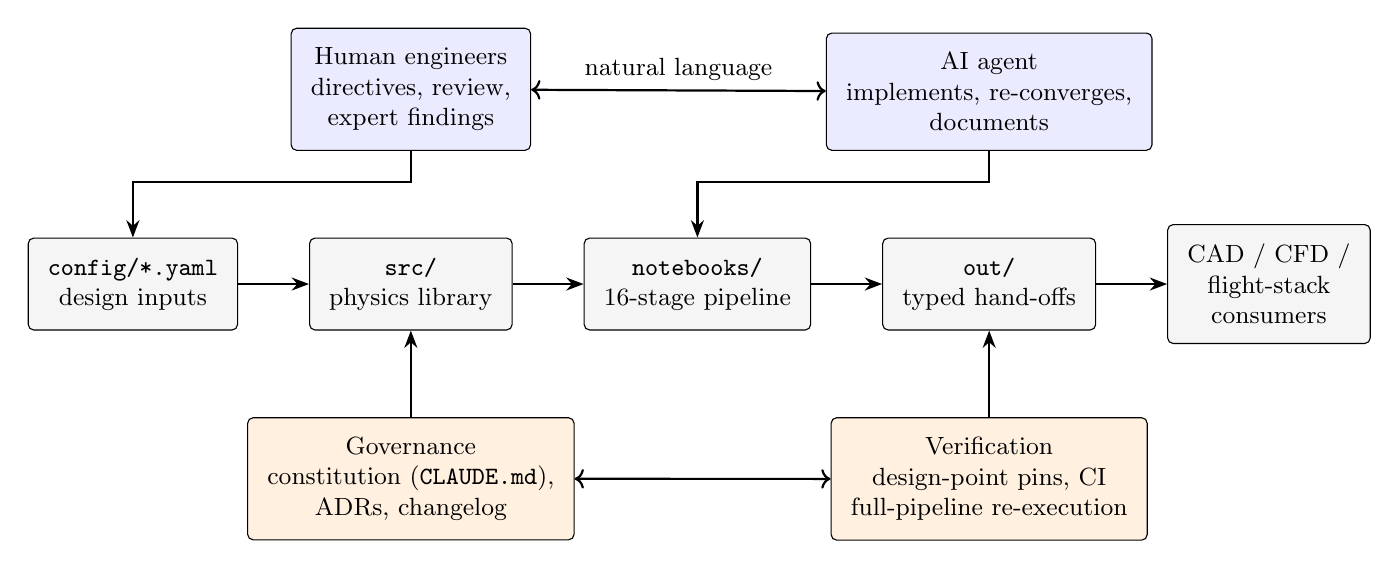
\begin{tikzpicture}[
  font=\small,
  node distance=5mm and 9mm,
  box/.style={draw, rounded corners=2pt, align=center, minimum height=8mm,
              inner sep=2.5mm, fill=gray!8},
  actor/.style={draw, align=center, minimum height=8mm, inner sep=2.5mm,
                fill=blue!8, rounded corners=2pt},
  gate/.style={draw, align=center, minimum height=8mm, inner sep=2.5mm,
               fill=orange!12, rounded corners=2pt},
  arr/.style={-{Stealth[length=2.2mm]}, thick}
]
% pipeline row
\node[box] (config) {\code{config/*.yaml}\\design inputs};
\node[box, right=of config] (src) {\code{src/}\\physics library};
\node[box, right=of src] (nb) {\code{notebooks/}\\16-stage pipeline};
\node[box, right=of nb] (out) {\code{out/}\\typed hand-offs};
\node[box, right=of out] (cfd) {CAD / CFD /\\flight-stack\\consumers};
\draw[arr] (config) -- (src);
\draw[arr] (src) -- (nb);
\draw[arr] (nb) -- (out);
\draw[arr] (out) -- (cfd);
% actors row
\node[actor, above=11mm of src] (human) {Human engineers\\directives, review,\\expert findings};
\node[actor, above=11mm of out] (ai) {AI agent\\implements, re-converges,\\documents};
\draw[arr, <->] (human) -- node[above]{natural language} (ai);
\draw[arr] (ai.south) -- ++(0,-4mm) -| (nb.north);
\draw[arr] (human.south) -- ++(0,-4mm) -| (config.north);
% gates row
\node[gate, below=11mm of src] (gov) {Governance\\constitution (\code{CLAUDE.md}),\\ADRs, changelog};
\node[gate, below=11mm of out] (ver) {Verification\\design-point pins, CI\\full-pipeline re-execution};
\draw[arr, <->] (gov) -- (ver);
\draw[arr] (gov.north) -- ++(0,4mm) -| (src.south);
\draw[arr] (ver.north) -- ++(0,4mm) -| (out.south);
\end{tikzpicture}%
}
\caption{The governed human--AI--repository loop. Engineering numbers
flow only left-to-right through the deterministic pipeline (top row);
the AI agent and human engineers modify the repository under the
governance and verification gates (bottom row).}
\label{fig:workflow}
\end{figure}

\subsection{The design repository as a one-way analysis pipeline}
\label{sec:pipeline}

All design knowledge lives in one repository with a strictly one-way
dataflow:
\begin{equation*}
\code{config/} \;\rightarrow\; \code{src/} \;\rightarrow\;
\code{notebooks/} \;\rightarrow\; \code{out/} \;\rightarrow\;
\text{CAD/CFD/flight-stack consumers.}
\end{equation*}
Every physical parameter --- mission times, aerodynamic limits,
battery properties, structural factors --- lives in commented YAML
configuration files with a written rationale; the Python physics
library contains \emph{no} magic numbers. Jupyter notebooks are thin
orchestration only (parameters, module calls, interpretation); all
physics, plotting, and reporting code lives in the importable library,
so the entire design is reproducible headlessly and testable by unit
tests. Each pipeline stage writes typed YAML/JSON hand-off files that
downstream stages read, and no stage ever writes back upstream. In the
case study this pipeline comprises sixteen notebook stages
(Table~\ref{tab:pipeline}), executed in dependency order.

This architecture is not incidental to the AI methodology --- it is
what makes an LLM agent safe to employ. Because the dataflow is
one-way and fully regenerable from \code{config/}, the agent can be
asked to re-converge the whole design after any change, and the effect
of the change is completely observable in the diff of the generated
hand-offs. Because notebooks are thin, the agent's edits concentrate
in ordinary, reviewable, unit-testable Python modules rather than in
opaque notebook state.

\begin{table}[htbp]
\centering
\caption{The sixteen-stage analysis pipeline of the case study. Each
stage writes typed hand-offs to \code{out/} that later stages consume;
stages 13--15 re-solve stages 4--6 with the frozen commercial hardware
without touching the conceptual outputs (no back-edge).}
\label{tab:pipeline}
\small
\begin{tabularx}{\textwidth}{@{}rlX@{}}
\toprule
\# & \textbf{Stage} & \textbf{Function} \\
\midrule
1 & Conceptual design & Mission sizing and iterative mass closure (MTOW, wing, power) \\
2 & Wing design & Airfoil selection and wing geometry \\
3 & Control vane design & Jet-vane sizing from hover thrust \\
4 & Aileron design & Cruise-phase roll authority (backup to vanes) \\
5 & Vibration isolation & FC/IMU and payload soft mounts vs.\ 1/rev rotor forcing \\
6 & Fuselage design & Packaging, center of gravity, drag trade \\
7 & Thermal design & ESC cold plate, vented battery bay, pack mission transient \\
8 & Vehicle solid model & Parametric CAD (STEP/STL export) \\
9 & Aerodynamic hand-off & Versioned JSON geometry contract for external VLM/BEMT analysis \\
10 & Mass properties & Inertia tensor, bill of materials, CG trim \\
11 & Wiring diagram & Generated electrical block diagram from the sizing result \\
12 & COTS selection & Deterministic component freeze against derived requirements \\
13--15 & As-selected re-solve & Stages 4--6 re-solved with frozen hardware masses/envelopes \\
16 & Design summary & Pure reader: design point, margins, standing findings \\
\bottomrule
\end{tabularx}
\end{table}

\subsection{Governance: a machine-readable project constitution}
\label{sec:governance}

The AI agent is steered by a \emph{project constitution} --- a
repository file (\code{CLAUDE.md}) that the agent loads at the start
of every working session and that encodes the engineering rules of the
program in plain language. In the case study it fixes, among others:

\begin{itemize}[nosep]
\item \textbf{No magic numbers}: every physical parameter lives in
  configuration with a commented rationale; numerical tolerances and
  named guard limits are the only exceptions.
\item \textbf{All physics in the library}: notebooks only set
  parameters, call modules, and interpret results.
\item \textbf{Conventions}: a single body-fixed axis convention
  (front--right--down) and unit discipline (SI in hand-offs and module
  interfaces; millimetres only inside CAD exports) applied uniformly
  across sizing, CAD, CFD, and documentation.
\item \textbf{Analysis-cost policy}: continuous integration validates
  CFD case \emph{setup} with a coarse smoke run only; converged CFD is
  never run in CI.
\item \textbf{Documentation duties}: every architecturally significant
  decision gets an architecture decision record (ADR); every tagged
  version gets a changelog entry.
\end{itemize}

Because the constitution is versioned alongside the code, the rules
evolve by the same review process as the design itself, and a new
human collaborator or a fresh AI session inherits identical
constraints. Design decisions are captured at decision time as ADRs
(status/context/decision/consequences); superseded decisions are never
rewritten but amended by new records, preserving the full reasoning
trail. In the case study the AI drafted each ADR as part of
implementing the corresponding change, and the human engineers
accepted or revised it in review --- eighteen ADRs over the program,
covering choices from ``all physics in \code{src/}'' to the propeller
blade section.

\subsection{Verification: making silent design drift impossible}
\label{sec:verification}

Three mechanisms ensure that neither the AI nor a human can move the
design unintentionally:

\paragraph{Design-point regression pins.} The converged design point
--- masses, geometry, control-surface torques, CFD reference values
--- is pinned in the test suite (147 test functions in the case
study). An \emph{intentional} design change must update the pins in
the same commit, which makes the diff itself the documentation of the
new design point; an \emph{unexpected} pin failure means the design
drifted and blocks the merge. This converts the classic LLM risk of
plausible-but-wrong output into a loud, reviewable event.

\paragraph{Full-pipeline continuous integration.} Every pull request
re-executes all sixteen notebook stages from scratch, runs the
regression and geometry tests (e.g., watertightness and unit checks on
exported CAD), and archives the regenerated hand-offs. On the main
branch, a coarse CFD smoke run additionally validates the OpenFOAM
case setup against the current geometry. Pushing a version tag
freezes a complete design snapshot (YAML hand-offs, STEP/STL geometry,
rendered notebooks) as an immutable release.

\paragraph{Cross-consumer consistency checks.} Values that must agree
across tool boundaries --- e.g., the CFD case's reference length,
area, and center of rotation versus the fuselage hand-off --- are
cross-checked by tests, so a design move that forgets a consumer fails
loudly. During the case study these checks caught, for example,
propulsion- and vane-CFD geometry that had silently drifted from the
converged design point, which was then re-sourced from the hand-offs
at run time.

A further discipline governs \emph{negative} results: margins that
come out unfavorable are recorded as pinned ``standing findings''
(reported by the final pipeline stage on every run) rather than tuned
away. Section~\ref{sec:results} lists the case study's standing
findings; methodologically, the point is that the AI is instructed to
surface unfavorable physics honestly, and the verification layer
prevents quiet re-tuning.

\subsection{Interaction protocol and provenance}
\label{sec:protocol}

Work proceeds in conversational sessions between an engineer and the
AI agent. The engineer's inputs are \emph{mission-level directives},
not code: representative examples from the case study include
``re-select the airfoil now that the stall-limited sizing is
honest,'' ``adopt a Clark~Y section for the propeller blade and
determine the rotation sense,'' ``fold the battery pack's internal
resistance into the closure consistently,'' and pasted findings from
an external design review. For each directive the agent:

\begin{enumerate}[nosep]
\item locates every discipline the change touches (sizing, geometry,
  control, thermal, CAD, CFD references, documentation);
\item implements the change in the physics library and configuration,
  with rationale comments;
\item re-executes the pipeline and re-converges the design point;
\item updates the regression pins, downstream consumer references, the
  ADR, and the changelog \emph{in the same commit}; and
\item opens a pull request that the human reviews and merges.
\end{enumerate}

Two provenance mechanisms make the AI's role auditable. First, every
AI-implemented commit carries a machine-readable co-authorship trailer
identifying the model, so the exact human/AI contribution split is
recoverable from the git history (Section~\ref{sec:process-results}).
Second, refactoring tasks are verified by \emph{byte-identical output
checks}: when the agent moved all notebook physics into the library
(ADR-0013 in the case study) and later split a pipeline stage
(ADR-0018), the generated hand-offs were verified byte-for-byte
unchanged before and after --- a strong guarantee that a structural
change carried no hidden design change.

The agent also maintains a persistent, human-readable memory of
project decisions and preferences across sessions (e.g., procurement
constraints such as preferring domestic retailers, or the standing
instruction to delete stale generated artifacts), complementing the
constitution with accumulated project context.

\subsection{Evidence-based iteration and external review}
\label{sec:iteration}

The design evolves through short, complete iterations: every
requirement change, model-fidelity improvement, or external finding
triggers a full re-convergence and a tagged snapshot, so the program
history is a sequence of internally consistent design points rather
than a single drifting draft. Three evidence channels feed this loop:

\begin{itemize}[nosep]
\item \textbf{Model refinement}: replacing an assumption with physics
  (e.g., an explicit structural member model replacing an area-density
  estimate; mission-transient battery heating replacing a steady-state
  vent check) and letting the closure re-converge honestly, even when
  the design gets heavier.
\item \textbf{Reality intrusion via procurement}: a deterministic
  commercial-component selection stage derives hard requirements from
  the converged design point and freezes the lightest feasible
  candidates; where no purchasable part matches an assumption (as
  happened with the case study's original fan diameter), the
  assumption --- not the report --- is amended, by ADR, and the design
  re-converged. A subsequent as-selected re-solve stage quantifies the
  gap between the conceptual closure and the frozen hardware without
  contaminating the conceptual baseline.
\item \textbf{Independent expert review}: domain experts outside the
  daily loop review the evolving design; their findings enter as
  directives and are traceable to the resulting ADRs. In the case
  study, external review contributed the semi-monocoque fuselage
  architecture, exposed a stall-speed inconsistency the automated
  checks could not see (a requirement silently unmet because a
  placeholder coefficient survived in one card), and prompted the
  battery internal-resistance accounting fix --- each of which moved
  the design point (Section~\ref{sec:results}).
\end{itemize}

Finally, the conceptual repository hands off to higher-fidelity
consumers through versioned, schema-validated contracts: a JSON
geometry hand-off (planform, body of revolution, control surfaces,
blade stations, moment reference point) feeds an external
vortex-lattice/blade-element analysis loop, while exported CAD and the
OpenFOAM cases support CFD on the same geometry. Schema evolution is
itself governed --- each field addition in the case study was a
reviewed, versioned, backward-compatible schema release, several of
them fixing real consumer-side integration faults (e.g., a missing
wing--body placement anchor that had put wing control points inside
the fuselage in the consumer's solver).

\section{Integrative Parameter Model of the Design Problem}
\label{sec:model}

Section~\ref{sec:method} described \emph{how} the human--AI--repository
loop is governed. This section describes \emph{what} it operates on:
the coupled parameter model of an electric VTOL UAV, the dimensioning
relations that implement it, and the constraint and verification checks
through which every iteration must pass. The two are complementary
contributions. The governance layer is what makes an AI agent safe to
employ; the integrative parameter model is what makes the agent
\emph{useful}, because it defines exactly which quantities a change
must be propagated to. An organization without heritage design tools
--- the situation of most emerging drone developers
(Section~\ref{sec:related}) --- needs both.

\subsection{Parameter taxonomy}
\label{sec:taxonomy}

The defining difficulty of electric VTOL conceptual design is that its
parameters do not separate cleanly into inputs and outputs. Wing area,
span, and airfoil are chosen by the designer, yet they are also
\emph{results} of the stall constraint at the converged weight; mission
endurance is a requirement, yet it is also what the closed battery mass
delivers. Treating such quantities as pure inputs is precisely the
error that produces internally inconsistent design cards --- as
happened in this project's own history (Section~\ref{sec:evolution}).
The model therefore classifies every quantity into one of five roles:

\begin{enumerate}[nosep,label=(\alph*)]
\item \textbf{Requirements} --- externally imposed and held fixed
  within an iteration: payload mass, mission segment durations, cruise
  speed, rate of climb, energy reserve, design ambient conditions.
\item \textbf{Free design parameters} --- the designer's (and the
  AI agent's) actual degrees of freedom: rotor diameter, blade count,
  pitch and solidity, aspect ratio, airfoil, thickness ratio,
  construction method and its structural knock-up factor, mass
  fractions, battery chemistry and cell count, component efficiencies.
\item \textbf{Coupled state variables} --- simultaneously input and
  output, resolved only by iteration: MTOW, battery mass, hover and
  cruise power, mission energy, wing area, span, and mean chord.
\item \textbf{Derived quantities} --- computed from the converged
  state, never configured: disk loading, induced and jet velocities,
  tip speed, dynamic pressures, lift-to-drag ratio, hover current,
  discharge C-rate, Joule heat, hinge moments, inertias, angular
  accelerations, pack temperature history.
\item \textbf{Constraints} --- inequalities the converged state must
  satisfy, each with an owner and a documented limit.
\end{enumerate}

Table~\ref{tab:params} lists the case-study instantiation. The
distinction is operationally important, not merely didactic: in the
repository, class (a) and (b) quantities live in commented
configuration files, class (c) and (d) quantities may only be produced
by the physics library, and class (e) quantities are asserted by the
test suite. The ``no magic numbers'' rule of
Section~\ref{sec:governance} is exactly the rule that keeps a class-(d)
quantity from being quietly hard-coded as if it were class-(a) --- the
failure mode behind the stall-speed inconsistency discussed later.

\begin{table}[htbp]
\centering
\caption{Parameter taxonomy of the case study. Requirements and free
parameters are configured with a written rationale; coupled and derived
quantities are computed only by the physics library; constraints are
asserted by the test suite.}
\label{tab:params}
\footnotesize
\begin{tabularx}{\textwidth}{@{}lXl@{}}
\toprule
\textbf{Role} & \textbf{Quantities (case study)} & \textbf{Lives in} \\
\midrule
Requirements &
$m_{\mathrm{pl}}=0.5$\,kg; $t_{\mathrm{hov}}=120$\,s,
$t_{\mathrm{tr}}=40$\,s, $t_{\mathrm{cr}}=900$\,s;
$V_{\mathrm{cr}}=20$\,m/s; RoC $=2.5$\,m/s;
$f_{\mathrm{res}}=1.20$; $\rho$, $T_\infty=40^{\circ}$C &
\code{config/} \\
\addlinespace
Free design parameters &
$D$, $N_b$, pitch, $\sigma$, FoM; AR, airfoil, $t/c$, $\lambda$,
$n_{\mathrm{ult}}$; construction method and $k$; $f_s,f_p,f_a,f_m$;
$e_{\mathrm{spec}}$, cell count $n_S$, $R_{\mathrm{pack}}$,
$f_{\mathrm{usable}}$; $\eta_p,\eta_m,\eta_{\mathrm{esc}}$ &
\code{config/} \\
\addlinespace
Coupled state variables &
$m_0$ (MTOW), $m_{\mathrm{batt}}$, $m_{\mathrm{wing}}$,
$P_{\mathrm{hov}}$, $P_{\mathrm{cr}}$, $E_{\mathrm{mis}}$,
$(W/S)^{\ast}$, $S$, $b$, $\bar{c}$ &
sizing loop \\
\addlinespace
Derived quantities &
$DL$, $v_i$, $V_{\mathrm{jet}}$, $q_{\mathrm{jet}}$,
$V_{\mathrm{tip}}$, $q_\infty$, $C_L$, $L/D$, $V_{\mathrm{MD}}$;
$I_{\mathrm{hov}}$, C-rate, $Q=I^2R_{\mathrm{pack}}$;
$M_{\mathrm{hinge}}$, $I_{xx}$, $\ddot\phi$, $\ddot\theta$;
$T_{\mathrm{batt}}(t)$, vent $\dot{m}$ &
\code{out/} hand-offs \\
\addlinespace
Constraints &
$V_{\mathrm{stall}}$, service ceiling, $T_{\mathrm{hov}}\le
T_{\max}$, C-rate $\le C_{\max}$, battery fraction, reserve energy,
$\ddot\theta\ge\ddot\theta_{\min}$, $T_{\mathrm{batt}}$ and
$T_{\mathrm{esc}}$ limits, packaging fit, CG range, $C_{D0}$ budget
(Table~\ref{tab:constraints}) &
test suite \\
\bottomrule
\end{tabularx}
\end{table}

\subsection{Parameter dependencies reported in the eVTOL literature}
\label{sec:dependencies}

Before mapping the couplings of the present vehicle it is worth
establishing which dependencies the eVTOL sizing literature already
treats as first-order, because the integrative model of
Section~\ref{sec:coupling} is a specialisation of them rather than a new
proposal. The consistent finding across eVTOL sizing studies is that
mass, geometry, aerodynamic performance, rotor loading, powertrain
choice, and transition feasibility feed back on one another rather than
being set independently, so sizing must be an iterative
multidisciplinary loop \citep{tyan2017,ugwueze2023,zhang2024evtol}. Two
consequences are specific to VTOL and recur throughout that literature.
First, the mission must be analysed at all critical points --- hover,
climb, transition, cruise, descent, and landing hover --- because
takeoff mass and energy capacity depend on every segment and not on
cruise alone \citep{tyan2017,ugwueze2022,hu2022}. Second, propulsion,
energy storage, and thermal management must be sized at component level,
since propeller, motor, ESC, and pack are strongly interdependent and
all scale with vehicle mass \citep{chahba2023,an2022,albamaestre2021}.

Table~\ref{tab:deps} collects the dependency structure in the
depends-on/drives form used by that literature, instantiated for a
single-propulsor tail-sitter. It is the qualitative statement of what
Fig.~\ref{fig:coupling} then makes concrete and
Section~\ref{sec:equations} quantifies.

\begin{table}[htbp]
\centering
\caption{Parameter dependencies for tail-sitter eVTOL conceptual design,
instantiated for a single-propulsor, battery-electric vehicle. The
depends-on/drives structure follows the eVTOL sizing literature cited in
each row; the parameter names are those of the present case study.}
\label{tab:deps}
\footnotesize
\begin{tabularx}{\textwidth}{@{}lXXX@{}}
\toprule
\textbf{Group} & \textbf{Primary parameters} & \textbf{Depends on} &
\textbf{Drives} \\
\midrule
Mission definition &
Payload, range/endurance, hover and transition budgets, cruise speed,
climb rate, ceiling, reserve &
Use case and top-level requirements \citep{he2025,lee2020} &
MTOW, stored energy, wing loading, rotor power
\citep{tyan2017,hu2022} \\
\addlinespace
Mass targets &
MTOW, structural/propulsion/avionics fractions, construction factor &
Mission energy, propulsion mass, airframe geometry, construction method
\citep{ugwueze2022,he2025} &
Required thrust, wing area, battery mass, transition feasibility
\citep{tyan2017,zhong2021} \\
\addlinespace
Wing and airframe geometry &
$W/S$, AR, span, area, chord, $C_{D0}$, $C_{L,\max}$, $L/D$ &
Cruise and stall constraints, transport/landing envelope, configuration
choice \citep{donateo2022,lee2020} &
Cruise power, stall margin, structural mass, transition corridor
\citep{hu2022,kubo2008} \\
\addlinespace
Rotor and propulsor &
Disk loading, diameter, blade count, solidity, pitch, thrust margin &
Hover power, takeoff weight, pack discharge capability
\citep{an2022,albamaestre2021,liu2024,qing2019} &
Hover efficiency, 1/rev forcing, jet dynamic pressure, control
authority, noise \citep{liu2024,govindarajan2018,sheng2015} \\
\addlinespace
Electric propulsion chain &
Motor and ESC rating, bus voltage, propeller--motor match &
Thrust and power required in every phase \citep{chahba2023} &
Propulsion mass, chain efficiency, thermal load, endurance
\citep{chahba2023} \\
\addlinespace
Battery system &
Specific energy and power, C-rate, DoD, pack resistance, voltage sag &
Mission profile, peak hover power, thermal limits
\citep{park2024,he2025} &
Battery mass, achievable hover/cruise power, cycle life, cooling need
\citep{park2024,zhao2024thermal} \\
\addlinespace
Thermal management &
Cooling path, airflow, vent and plate area, allowable temperature &
Heat generation, C-rate, hover duration
\citep{park2024,zhao2024thermal} &
Effective specific energy, thermal-system mass, degradation, safety
margin \citep{park2024,zhao2024thermal} \\
\addlinespace
Transition and control &
Pitch schedule, actuator and rate limits, vane and aileron authority,
time delay &
Airframe geometry, propulsion authority, wing aerodynamics
\citep{zhong2021,mcintosh2024,li2020} &
Feasible transition time, altitude loss, robustness, effector sizing
\citep{li2020,cong2024,banazadeh2016,marvakov2021} \\
\addlinespace
Volume and packaging integration &
Bay stack, pack volume, fuselage envelope, CG range &
Component envelopes, structural architecture, landing footprint
\citep{lee2020,govindarajan2018} &
Achievable pack size, static margin, structural mass
\citep{ugwueze2023} \\
\bottomrule
\end{tabularx}
\end{table}

Three findings from that literature are worth stating explicitly
because they bear on the constraint set of
Section~\ref{sec:checks}. Battery sizing constrained only by constant
specific energy is insufficient: voltage drop, temperature, depth of
discharge, and C-rate all belong in the conceptual loop
\citep{park2024}, and in the highest-power segments power density can
matter more than energy density \citep{thu2025}. Thermal management can
change feasibility outright rather than merely adding mass, since longer
hover demands substantially heavier cooling \citep{zhao2024thermal}.
And transition is a sizing constraint, not only a control problem:
imposing a minimum-transition-time constraint during sizing has been
shown to reduce takeoff weight by nearly 5\% relative to an unconstrained
initial design \citep{cong2024}, while the transition corridor widens
with available propulsive power and narrows with weight
\citep{tang2018,zhong2021}. For small battery-powered tail-sitters
specifically, higher battery mass fraction and lower wing loading
improve achievable performance \citep{wang2016}, and simultaneous
optimisation of wing loading, aspect ratio, and battery fraction against
energy consumption has been reported to raise the payload fraction
materially \citep{cinar2023}.

\subsection{The coupling map}
\label{sec:coupling}

Fig.~\ref{fig:coupling} is the integrative model: it shows which
factors influence which, and where the loops are. It follows the
depends-on/drives structure of Table~\ref{tab:deps}, and is drawn in the
sizing-flow form so that the primary path, the constraint and feedback
edges, and the dominant iterative loop are visually distinct. Two
circular dependencies dominate and must be resolved simultaneously.

The \textbf{closure loop} (heavy boxes, centre row) is the classical
electric-aircraft circularity: the battery is the heaviest single item,
its mass follows from mission energy, mission energy follows from
power, power follows from weight, and weight includes the battery.
Because the structural and subsystem masses are expressed as fractions
of MTOW, the loop admits an analytical step for weight given battery
mass, and the iteration reduces to a fixed point in
$m_{\mathrm{batt}}$ alone --- a contraction, because doubling the
vehicle weight does not double the required energy.

The \textbf{wing loop} enters through the stall constraint. The design
wing loading is bounded above by
$(W/S)_{\mathrm{stall}}=\tfrac{1}{2}\rho V_{\mathrm{stall}}^{2}
C_{L,\max}$, so wing area is set by weight, and weight is influenced by
wing mass. This is why the airfoil choice --- nominally a free
parameter --- propagates all the way into vehicle geometry: raising
$C_{L,\max}$ raises the admissible wing loading and \emph{shrinks} the
wing at constant weight. It is also why $C_{L,\max}$ must track the
airfoil selection in the same change; a stale value silently relaxes a
requirement rather than failing a test.

Two further couplings deserve note because they are easy to miss in a
sequential workflow, and both bit this project:

\begin{itemize}[nosep]
\item \textbf{Rotor diameter is a mass parameter, not only a
  propulsion parameter.} Disk loading is derived, $DL=m_0g/(\pi
  D^{2}/4)$, so a diameter change moves hover power, hence energy,
  hence battery mass, hence MTOW --- and simultaneously moves jet
  dynamic pressure, hence control-vane authority, hinge moments, servo
  torque requirement, and the 1/rev vibration forcing frequency.
\item \textbf{Pack internal resistance couples the thermal model to
  the mass closure.} $R_{\mathrm{pack}}$ sets both the Joule heat
  $I^{2}R$ that the battery bay must vent and the discharge efficiency
  $\eta_{\mathrm{bat}}$ that appears in the battery-mass relation.
  Treating the two independently permits a design that is thermally
  sized for a resistive pack while being mass-sized for an ideal one.
\end{itemize}

\begin{sidewaysfigure}
\centering
\hyphenpenalty=10000 \exhyphenpenalty=10000
\resizebox{\textheight}{!}{%
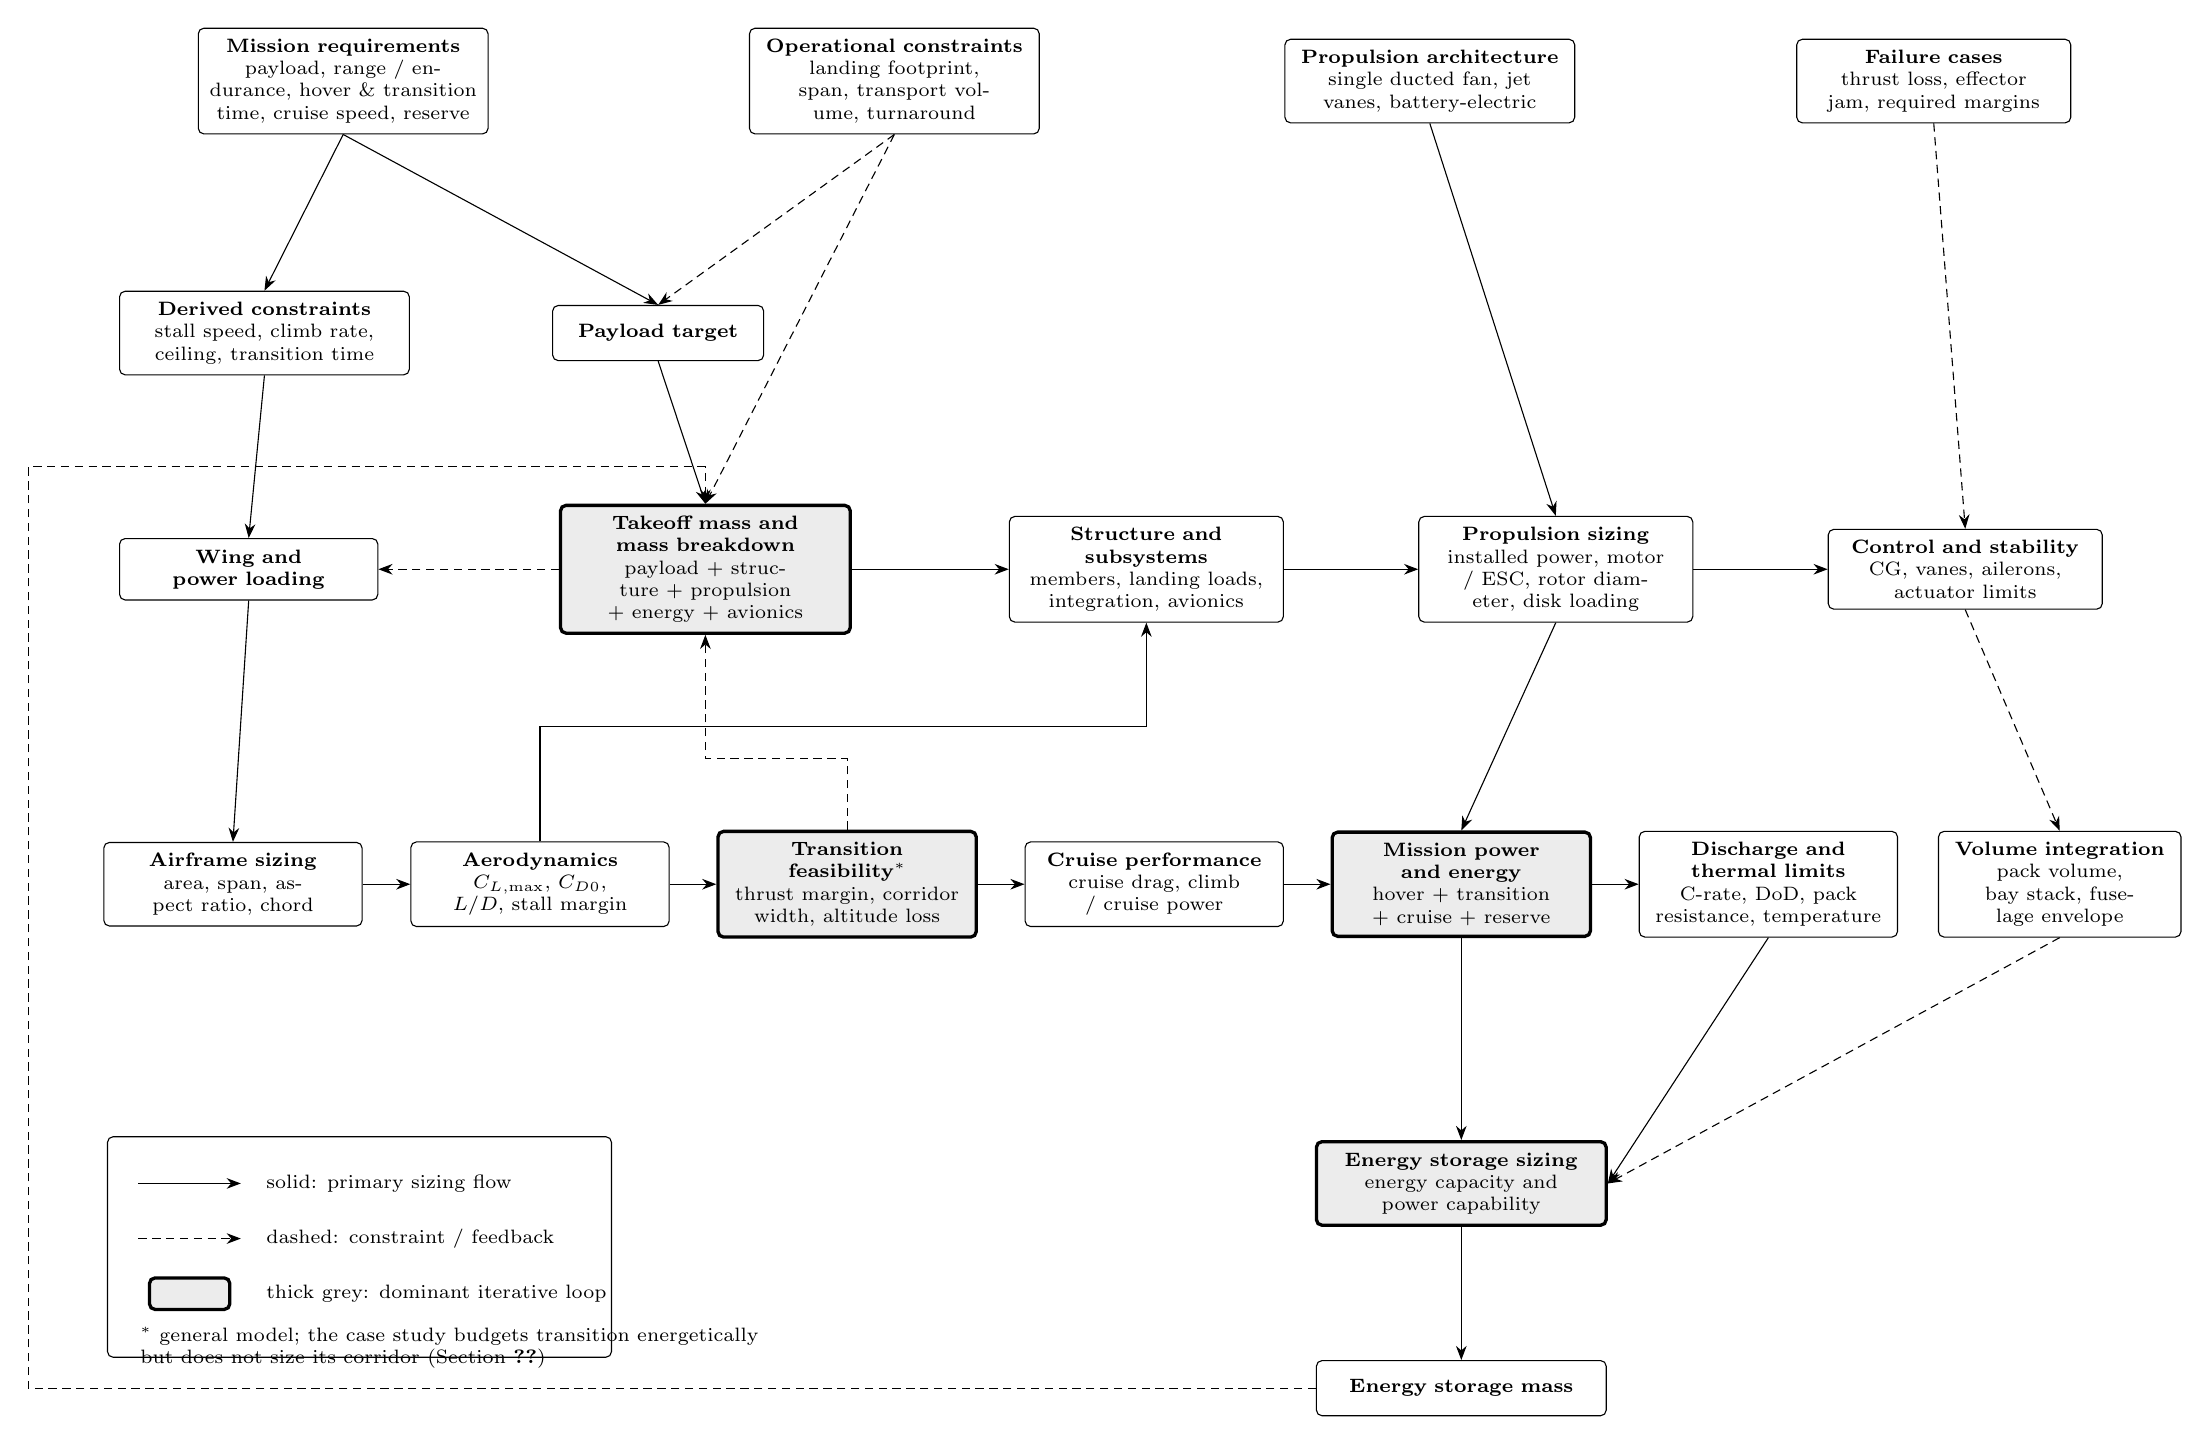
\begin{tikzpicture}[
  font=\scriptsize,
  bx/.style={draw, rounded corners=2pt, align=center, inner sep=1.4mm,
             minimum height=7mm, text width=30mm, fill=white},
  loop/.style={bx, very thick, fill=gray!15},
  a/.style={-{Stealth[length=1.8mm]}},
  fb/.style={-{Stealth[length=1.8mm]}, densely dashed}
]

% ================= band 0: external inputs =================
\node[bx, text width=34mm] (mis) at ( 4.4, 0.0)
  {\textbf{Mission requirements}\\payload, range / endurance,
   hover \& transition time, cruise speed, reserve};
\node[bx, text width=34mm] (ops) at (11.4, 0.0)
  {\textbf{Operational constraints}\\landing footprint, span,
   transport volume, turnaround};
\node[bx, text width=34mm] (arch) at (18.2, 0.0)
  {\textbf{Propulsion architecture}\\single ducted fan, jet vanes,
   battery-electric};
\node[bx, text width=32mm] (fail) at (24.6, 0.0)
  {\textbf{Failure cases}\\thrust loss, effector jam,
   required margins};

% ================= band 1: derived constraints / payload =================
\node[bx, text width=34mm] (dcon) at ( 3.4,-3.2)
  {\textbf{Derived constraints}\\stall speed, climb rate,
   ceiling, transition time};
\node[bx, text width=24mm] (pl) at ( 8.4,-3.2) {\textbf{Payload target}};

% ================= band 2: loadings, mass, subsystems =================
\node[bx] (wl) at ( 3.2,-6.2)
  {\textbf{Wing and power loading}};
\node[loop, text width=34mm] (m0) at ( 9.0,-6.2)
  {\textbf{Takeoff mass and mass breakdown}\\payload + structure +
   propulsion + energy + avionics};
\node[bx, text width=32mm] (str) at (14.6,-6.2)
  {\textbf{Structure and subsystems}\\members, landing loads,
   integration, avionics};
\node[bx, text width=32mm] (prop) at (19.8,-6.2)
  {\textbf{Propulsion sizing}\\installed power, motor / ESC,
   rotor diameter, disk loading};
\node[bx, text width=32mm] (ctl) at (25.0,-6.2)
  {\textbf{Control and stability}\\CG, vanes, ailerons,
   actuator limits};

% ================= band 3: performance chain =================
\node[bx] (wing) at ( 3.0,-10.2)
  {\textbf{Airframe sizing}\\area, span, aspect ratio, chord};
\node[bx] (aero) at ( 6.9,-10.2)
  {\textbf{Aerodynamics}\\$C_{L,\max}$, $C_{D0}$,
   $L/D$, stall margin};
\node[loop] (tr) at (10.8,-10.2)
  {\textbf{Transition feasibility}$^{\ast}$\\thrust margin,
   corridor width, altitude loss};
\node[bx] (cr) at (14.7,-10.2)
  {\textbf{Cruise performance}\\cruise drag,
   climb / cruise power};
\node[loop] (en) at (18.6,-10.2)
  {\textbf{Mission power and energy}\\hover + transition
   + cruise + reserve};
\node[bx] (lim) at (22.5,-10.2)
  {\textbf{Discharge and thermal limits}\\C-rate, DoD,
   pack resistance, temperature};
\node[bx, text width=28mm] (vol) at (26.2,-10.2)
  {\textbf{Volume integration}\\pack volume, bay stack,
   fuselage envelope};

% ================= band 4/5: energy storage =================
\node[loop, text width=34mm] (es) at (18.6,-14.0)
  {\textbf{Energy storage sizing}\\energy capacity and
   power capability};
\node[bx, text width=34mm] (esm) at (18.6,-16.6)
  {\textbf{Energy storage mass}};

% ================= primary sizing flow =================
\draw[a] (mis.south)  -- (dcon.north);
\draw[a] (mis.south)  -- (pl.north);
\draw[a] (arch.south) -- (prop.north);
\draw[a] (dcon.south) -- (wl.north);
\draw[a] (pl.south)   -- (m0.north);
\draw[a] (m0)   -- (str);
\draw[a] (str)  -- (prop);
\draw[a] (prop) -- (ctl);
\draw[a] (wl.south)   -- (wing.north);
\draw[a] (wing) -- (aero);
\draw[a] (aero) -- (tr);
\draw[a] (tr)   -- (cr);
\draw[a] (cr)   -- (en);
\draw[a] (en)   -- (lim);
\draw[a] (prop.south) -- (en.north);
\draw[a] (en.south)   -- (es.north);
\draw[a] (lim.south)  -- (es.east);
\draw[a] (es.south)   -- (esm.north);
% wing geometry informs the structural member model
\draw[a] (aero.north) -- (6.9,-8.2) -- (14.6,-8.2) -- (str.south);

% ================= constraints and feedback =================
\draw[fb] (ops.south)  -- (pl.north);
\draw[fb] (ops.south)  -- (m0.north);
\draw[fb] (fail.south) -- (ctl.north);
\draw[fb] (ctl.south)  -- (vol.north);
\draw[fb] (vol.south)  -- (es.east);
% converged mass drives the loadings back
\draw[fb] (m0.west) -- (wl.east);
% transition feasibility constrains the mass breakdown
\draw[fb] (tr.north) -- (10.8,-8.6) -- (9.0,-8.6) -- (m0.south);
% the dominant loop closes: energy storage mass re-enters the mass breakdown
\draw[fb] (esm.west) -- (0.4,-16.6) -- (0.4,-4.9) -- (9.0,-4.9) -- (m0.north);

% ================= legend =================
\begin{scope}
  \node[draw, rounded corners=2pt, minimum width=64mm, minimum height=28mm,
        anchor=north west] at (1.4,-13.4) {};
  \draw[a] (1.8,-14.0) -- (3.1,-14.0);
  \node[anchor=west] at (3.3,-14.0) {solid: primary sizing flow};
  \draw[fb] (1.8,-14.7) -- (3.1,-14.7);
  \node[anchor=west] at (3.3,-14.7) {dashed: constraint / feedback};
  \node[loop, text width=9mm, minimum height=4mm, inner sep=0.6mm]
        at (2.45,-15.4) {};
  \node[anchor=west] at (3.3,-15.4) {thick grey: dominant iterative loop};
  \node[anchor=north west, align=left] at (1.7,-15.7)
    {$^{\ast}$ general model; the case study budgets transition
     energetically\\ but does not size its corridor
     (Section~\ref{sec:discussion})};
\end{scope}
\end{tikzpicture}%
}
\caption{Integrative sizing and coupling map for tail-sitter eVTOL
conceptual design, in the depends-on/drives structure of
Table~\ref{tab:deps} and instantiated for the case-study vehicle
(diagram topology after \c{C}.~U\c{c}ler). Solid edges are the primary
sizing flow; dashed edges are constraints and feedback; the four heavy
grey boxes are the dominant iterative loop, which closes when the energy
storage mass re-enters the mass breakdown. Representative edges are
drawn; the complete dependency set is enforced in code.}
\label{fig:coupling}
\end{sidewaysfigure}

\subsection{Dimensioning relations}
\label{sec:equations}

The relations below are the conceptual-level physics the pipeline
implements. They are deliberately first-order and transparent: the
methodology's claim is not fidelity but traceability, and every symbol
resolves either to a configured parameter with a written rationale or
to another equation in this set. They are used in the form collected by
\citet{poelma2024}, which consolidates the Gudmundsson/Sadraey
constraint-diagram relations, the Raymer weight regressions, and the
VTOL power-to-weight formulation of \citet{tyan2017} into one
conceptual-sizing procedure for electric VTOL UAVs; the section
references the primary sources alongside.

\paragraph{Wing loading and thrust loading.} With a parabolic drag
polar $C_D=C_{D0}+kC_L^{2}$, $k=1/(\pi\,\mathrm{AR}\,e)$, and
$q=\tfrac{1}{2}\rho V^{2}$, each flight phase gives a required thrust
loading as a function of wing loading \citep{gudmundsson2014,sadraey2013}:
\begin{align}
\text{cruise:}\quad
  \frac{T}{W} &= \frac{q\,C_{D0}}{W/S} + \frac{k\,(W/S)}{q},
  \qquad q=\tfrac{1}{2}\rho V_{\mathrm{cr}}^{2},
  \label{eq:smd}\\
\text{climb:}\quad
  \frac{T}{W} &= \frac{\mathrm{RoC}}{V} + \frac{q\,C_{D0}}{W/S}
                 + \frac{k\,(W/S)}{q},
  \qquad V=\sqrt{\frac{2}{\rho}\sqrt{\frac{k}{3C_{D0}}}\,\frac{W}{S}},
  \label{eq:climb}\\
\text{ceiling:}\quad
  \frac{T}{W} &= \frac{\mathrm{RoC}_{\mathrm{ceil}}}{V_{\mathrm{mp}}}
                 + 4\sqrt{\frac{k\,C_{D0}}{3}},
  \label{eq:ceiling}\\
\text{max speed:}\quad
  \frac{T}{W} &= \frac{\rho V_{\max}^{2}C_{D0}}{2\,(W/S)}
                 + \frac{2k\,(W/S)}{\rho V_{\max}^{2}} .
  \label{eq:vmax}
\end{align}
The stall requirement is a vertical boundary rather than a curve,
\begin{equation}
\left(\frac{W}{S}\right)_{\mathrm{stall}}
  = \tfrac{1}{2}\,\rho\,V_{\mathrm{stall}}^{2}\,C_{L,\max},
\label{eq:stall}
\end{equation}
and the design point minimises the upper envelope of
Eqs.~(\ref{eq:smd})--(\ref{eq:vmax}) inside the feasible region,
\begin{equation}
\begin{aligned}
(W/S)^{\ast}
  &= \operatorname*{arg\,min}_{\,W/S\,\le\,(W/S)_{\mathrm{stall}}}\;
     \max_{\text{phases}} \frac{T}{W}\!\left(\frac{W}{S}\right),\\[2pt]
(T/W)^{\ast}
  &= \max_{\text{phases}}\frac{T}{W}\Big((W/S)^{\ast}\Big),
\end{aligned}
\label{eq:designpoint}
\end{equation}
which simultaneously minimises propulsion size and battery mass. Wing
geometry then follows from the converged weight,
\begin{equation}
S = \frac{m_0\,g}{(W/S)^{\ast}},
\qquad
b = \sqrt{\mathrm{AR}\cdot S},
\qquad
\bar{c} = \frac{S}{b},
\label{eq:winggeom}
\end{equation}
with wing structural mass from Raymer's general-aviation regression
\citep{raymer2018}, scaled by a material factor
$k_{\mathrm{mat}}$ ($0.70$ for CFRP):
\begin{equation}
m_{\mathrm{wing}} = k_{\mathrm{mat}}\;0.036\,
  S^{0.758}\,
  \left(\frac{\mathrm{AR}}{\cos^{2}\Lambda}\right)^{0.6}
  q^{0.006}\,\lambda^{0.04}
  \left(\frac{100\,t/c}{\cos\Lambda}\right)^{-0.3}
  \left(n_{\mathrm{ult}}W_0\right)^{0.49},
\label{eq:raymer}
\end{equation}
evaluated in the imperial units of the original regression and
converted back to SI.

\paragraph{Hover and vertical flight.} For a tail-sitter the single
rotor carries the entire weight, so disk loading is derived rather than
chosen:
\begin{equation}
DL = \frac{m_0\,g}{\pi D^{2}/4}.
\label{eq:dl}
\end{equation}
Momentum (actuator-disk) theory with a figure of merit gives the hover
shaft power, and the vertical-climb case adds blade profile drag and
the parasite drag of fuselage and wing in the vertical airstream:
\begin{align}
\left(\frac{P}{W}\right)_{\mathrm{hov}}
  &= \frac{1}{\mathrm{FoM}}\sqrt{\frac{DL}{2\rho}},
  \label{eq:hover}\\
\left(\frac{P}{W}\right)_{\mathrm{climb}}
  &= \underbrace{\frac{\mathrm{RoC}}{2}
     + \frac{1}{2}\sqrt{\mathrm{RoC}^{2}+\frac{2\,DL}{\rho}}}
     _{\text{induced}+\text{climb}}
   + \underbrace{\frac{\rho\,V_{\mathrm{tip}}^{3}\,\sigma\,C_{d}}{8\,DL}}
     _{\text{blade profile}}
   \notag \\
  &\qquad
   + \underbrace{\frac{\rho\,\mathrm{RoC}^{3}}{DL}}_{\text{fuselage}}
   + \underbrace{\frac{\rho\,\mathrm{RoC}^{3}}{S_{r}\,(W/S)}}_{\text{wing}},
  \label{eq:vclimb}
\end{align}
with tip speed from an empirical rotor speed--diameter relation,
$N = k_{\mathrm{rpm}}D^{\,n}$ and
$V_{\mathrm{tip}} = \pi N D/60$. Electrical power adds the drive chain
and the continuous avionics (hotel) load,
\begin{equation}
P_{\mathrm{hov}}
  = \frac{(P/W)_{\mathrm{vtol}}\;m_0\,g}
         {\eta_m\,\eta_{\mathrm{esc}}} + P_{\mathrm{hotel}},
\qquad
(P/W)_{\mathrm{vtol}} = \max\!\left[
  \left(\tfrac{P}{W}\right)_{\mathrm{hov}},
  \left(\tfrac{P}{W}\right)_{\mathrm{climb}}\right],
\label{eq:phov}
\end{equation}
while wing-borne cruise power uses the lift-to-drag model,
\begin{equation}
P_{\mathrm{cr}} = \frac{m_0\,g\,V_{\mathrm{cr}}}{(L/D)\;\eta_{\mathrm{tot}}}
                  + P_{\mathrm{hotel}},
\qquad
\eta_{\mathrm{tot}} = \eta_p\,\eta_m\,\eta_{\mathrm{esc}}.
\label{eq:pcr}
\end{equation}

\paragraph{Energy, battery, and mass closure.} Transitions are billed
conservatively at hover power, and the reserve is a multiplier on the
total:
\begin{equation}
E_{\mathrm{mis}} = \frac{f_{\mathrm{res}}}{3600}\Big[
  P_{\mathrm{hov}}\,(t_{\mathrm{hov}}+t_{\mathrm{tr}})
  + P_{\mathrm{cr}}\,t_{\mathrm{cr}}\Big].
\label{eq:energy}
\end{equation}
Battery mass follows from pack-level specific energy, discharge
efficiency, and usable depth of discharge \citep{tyan2017}, and MTOW
closes analytically against the mass fractions:
\begin{equation}
m_{\mathrm{batt}} = \frac{E_{\mathrm{mis}}}
  {e_{\mathrm{spec}}\;\eta_{\mathrm{bat}}\;f_{\mathrm{usable}}},
\qquad
m_0 = \frac{m_{\mathrm{pl}} + m_{\mathrm{batt}}}
           {1 - (f_s + f_p + f_a + f_m)} .
\label{eq:closure}
\end{equation}
Equations~(\ref{eq:dl})--(\ref{eq:closure}) are the closure loop of
Fig.~\ref{fig:coupling}, iterated to
$|m_{\mathrm{batt}}^{(i+1)}-m_{\mathrm{batt}}^{(i)}| < \varepsilon$.
The structural fraction is scaled by the construction method,
$f_s = k\,f_{s,\mathrm{base}}$, which makes $k$ the single most
sensitive mass parameter in the model. The converged operating point
gives the peak discharge rate and the pack current used by the
electrical and thermal stages:
\begin{equation}
C_{\mathrm{peak}}
  = \frac{\max(P_{\mathrm{hov}},P_{\mathrm{cr}})}
         {m_{\mathrm{batt}}\,e_{\mathrm{spec}}},
\qquad
I_{\mathrm{hov}} = \frac{P_{\mathrm{hov}}}{n_S\,V_{\mathrm{cell}}} .
\label{eq:crate}
\end{equation}

\paragraph{Control authority.} Jet-vane authority is sized from hover
thrust. With $T=m_0g$ the induced velocity, fully developed jet
velocity, and vane dynamic pressure are
\begin{equation}
v_i = \sqrt{\frac{T}{2\rho A}},
\qquad V_{\mathrm{jet}} = 2v_i,
\qquad q_{\mathrm{jet}} = \tfrac{1}{2}\rho V_{\mathrm{jet}}^{2}
  = \frac{T}{A},
\label{eq:jet}
\end{equation}
so vane force, control moment, angular acceleration, and the servo
torque requirement follow as
\begin{equation}
F_v = q_{\mathrm{jet}} S_v C_{l\alpha}\delta,
\qquad
\ddot\theta = \frac{n_v F_v \ell}{I_{\theta}},
\qquad
M_{\mathrm{hinge}} = q_{\mathrm{jet}} S_v c_v C_{h},
\qquad
M_{\mathrm{servo}} = M_{\mathrm{hinge}}\,\mathrm{SF}\,f_m .
\label{eq:vane}
\end{equation}
Equation~(\ref{eq:jet}) exposes why a second roll effector is
structurally necessary rather than merely prudent: $q_{\mathrm{jet}} =
T/A$ is \emph{linear} in thrust, and cruise thrust is smaller than
hover thrust by roughly the factor $L/D$, so vane authority collapses
in cruise. Ailerons instead use free-stream dynamic pressure, with
Glauert flap effectiveness
$\tau = 1-(\theta_f-\sin\theta_f)/\pi$,
$\theta_f = \arccos(2c_f/c-1)$:
\begin{equation}
\ddot\phi = \frac{2\,q_\infty\,S_a\,(C_{L\alpha}\tau)\,\delta\,y_a}
                 {I_{xx}} .
\label{eq:aileron}
\end{equation}
The two effectors are therefore complementary by construction: each is
strongest exactly where the other is weakest, and both are checked
against the same authority floor $\ddot\theta_{\min}$.

\paragraph{Thermal paths.} The two hover heat loads are derived from
the converged operating point, not configured:
$Q_{\mathrm{esc}} = P_{\mathrm{hov}}(1-\eta_{\mathrm{esc}})$ and
$Q_{\mathrm{batt}} = I_{\mathrm{hov}}^{2}R_{\mathrm{pack}}$. Forced
convection on the inflow-washed cold plate and the vented battery bay
give the steady sizing relations
\begin{equation}
T_{\mathrm{plate}}(A) = T_\infty + \frac{Q_{\mathrm{esc}}}{C_h A^{3/4}},
\qquad
\Delta T_{\mathrm{air}} = \frac{Q_{\mathrm{batt}}}{\dot{m}\,c_p},
\qquad
\dot{m} = \rho\,V_{\mathrm{vent}}\,A_{\mathrm{vent}} .
\label{eq:thermalss}
\end{equation}
Because the vent check is air-side only, it cannot see the pack's own
temperature rise; a lumped-capacitance mission transient with
$C_{\mathrm{th}} = m_{\mathrm{batt}}c_{p,\mathrm{pack}}$ and
$\tau = C_{\mathrm{th}}/(UA)$ is therefore integrated over the two
vertical legs and the cruise segment between them,
\begin{equation}
\Delta T_{\mathrm{leg}} = \frac{Q_{\mathrm{hov}}\,t_{\mathrm{leg}}}
                               {C_{\mathrm{th}}},
\qquad
T(t) = T_{\mathrm{ss}} + \big(T_0-T_{\mathrm{ss}}\big)e^{-t/\tau},
\qquad
T_{\mathrm{ss}} = T_\infty + \frac{Q_{\mathrm{cr}}}{UA},
\label{eq:transient}
\end{equation}
and evaluated at a bracket of pack resistances. This is the check that
exposed the design's second standing finding
(Section~\ref{sec:design-results}).

\subsection{Constraints and the iteration check flow}
\label{sec:checks}

Table~\ref{tab:constraints} lists the constraint set with its source
and enforcement point. Two properties matter methodologically. First,
each limit is \emph{configured with a rationale} while the quantity
compared against it is \emph{derived} --- so a design change cannot
relax a requirement by accident, only by an explicit, reviewable edit
to a configuration file. Second, each constraint has a named
enforcement mechanism, ranging from a hard exception that aborts the
sizing loop to a reported margin that is allowed to be negative
provided it is carried as a standing finding.

\begin{table}[htbp]
\centering
\caption{Constraint set of the case study, with the enforcement
mechanism for each. ``Hard'' aborts the pipeline; ``pinned'' is
asserted by the regression suite; ``reported'' is a margin that may be
negative only as a documented standing finding.}
\label{tab:constraints}
\footnotesize
\begin{tabularx}{\textwidth}{@{}Xllc@{}}
\toprule
\textbf{Constraint} & \textbf{Limit (case study)} &
\textbf{Owner} & \textbf{Type} \\
\midrule
Battery fraction (closure divergence guard) &
$m_{\mathrm{batt}}/m_0 \le 0.60$ & sizing loop & hard \\
Hover thrust within COTS rotor capability &
$T_{\mathrm{hov}} \le T_{\max}=35$\,N & sizing study & hard \\
Mass-fraction sum consistency &
$\sum f_i + f_{\mathrm{batt}} + f_{\mathrm{pl}} = 1$ &
sizing loop & pinned \\
Stall speed &
$V_{\mathrm{stall}} \le 12$\,m/s via Eq.~(\ref{eq:stall}) &
wing stage & pinned \\
Service ceiling &
$h \ge 3000$\,m at $\mathrm{RoC}=0.5$\,m/s &
size matching & pinned \\
Peak discharge rate &
$C_{\mathrm{peak}} \le 25$\,C & sizing loop & pinned \\
Mission energy reserve &
$f_{\mathrm{res}} = 1.20$ & sizing loop & pinned \\
Angular acceleration, all axes, hover and cruise &
$\ddot\theta \ge 30^{\circ}$/s$^{2}$ & vane, aileron stages & pinned \\
Vibration isolation window at 1/rev &
transmissibility target at $\sim$204\,Hz & isolation stage & pinned \\
ESC junction temperature &
$T_{\mathrm{esc}}$ limit at $T_\infty=40^{\circ}$C &
thermal stage & reported \\
Battery pack temperature (steady and transient) &
$T_{\mathrm{batt}} \le 60^{\circ}$C & thermal stage & reported \\
Packaging fit, bay stack, CG range &
rigid-part axial lengths, static margin &
fuselage stages & pinned \\
Cruise drag budget &
$C_{D0} \le 0.025$ (build-up vs.\ configured) &
fuselage stage & reported \\
Mass allocation per component group &
as-selected mass $\le$ fraction allocation &
freeze stage & reported \\
Cross-consumer reference consistency &
CFD $l_{\mathrm{ref}}$, $A_{\mathrm{ref}}$, CofR vs.\ hand-off &
test suite & pinned \\
\bottomrule
\end{tabularx}
\end{table}

Fig.~\ref{fig:checkflow} traces how these checks are actually used
within one iteration. The flow has three distinct failure exits, and
keeping them distinct is what makes the framework usable as a review
instrument. A \emph{hard} failure means the concept does not close at
all and the sizing loop refuses to produce a number --- the response is
to change a free parameter or, where the assumption itself was wrong,
to amend it by decision record. A \emph{pinned} failure means the
design moved: if the move was intended, the pins, downstream consumer
references, decision record, and changelog are updated in the same
commit, so the diff documents the new design point; if it was not, the
merge is blocked because the design has drifted silently. A
\emph{reported} negative margin does not block anything, but it cannot
be silenced either: it is emitted by the final pipeline stage on every
run until it is retired.

\begin{figure}[htbp]
\centering
\resizebox{0.90\textwidth}{!}{%
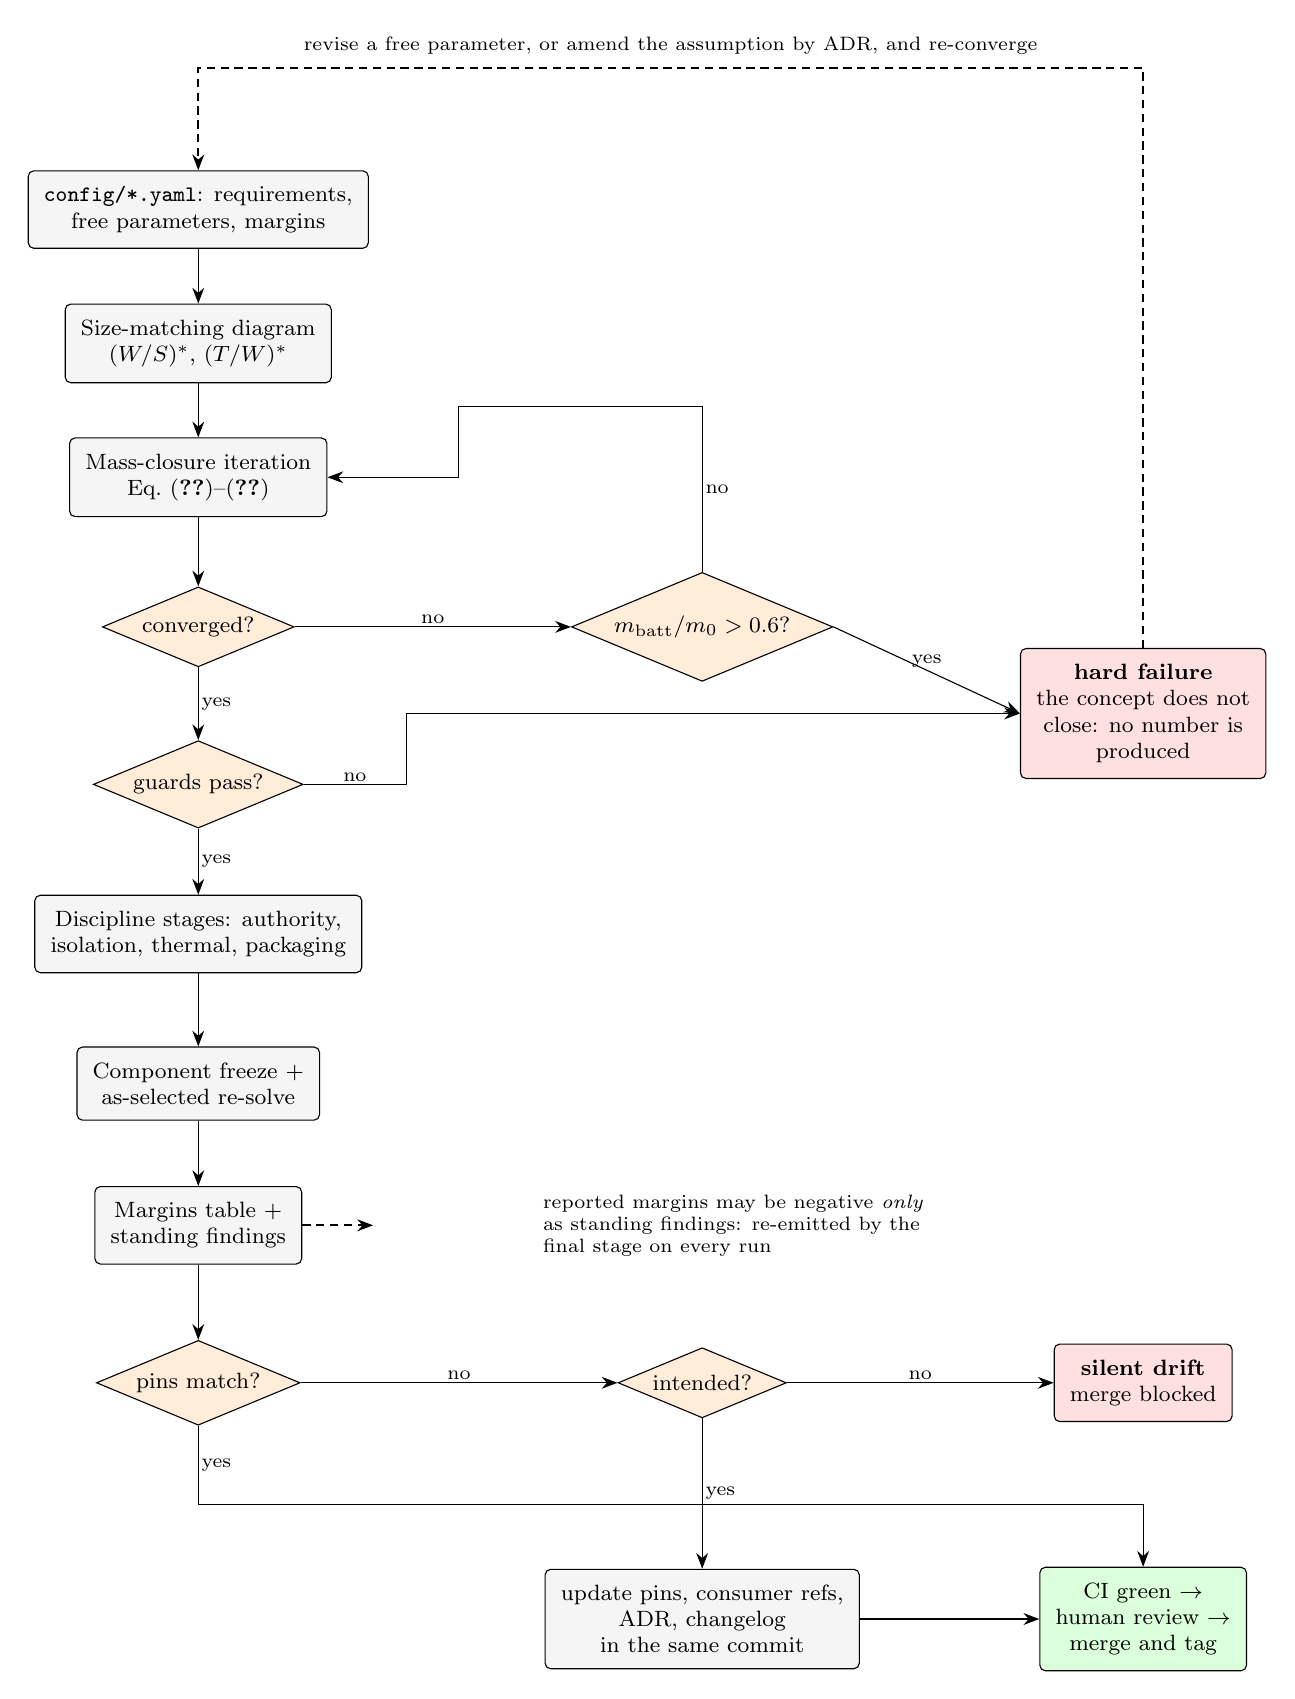
\begin{tikzpicture}[
  font=\footnotesize,
  proc/.style={draw, rounded corners=2pt, align=center, inner sep=2mm,
               minimum height=9mm, fill=gray!8},
  dec/.style={draw, diamond, aspect=2.4, align=center, inner sep=0.6mm,
              fill=orange!15},
  bad/.style={draw, rounded corners=2pt, align=center, inner sep=2mm,
              fill=red!12, minimum height=9mm},
  good/.style={draw, rounded corners=2pt, align=center, inner sep=2mm,
               fill=green!14, minimum height=9mm},
  a/.style={-{Stealth[length=2mm]}},
  fb/.style={-{Stealth[length=2mm]}, densely dashed, thick},
  el/.style={font=\scriptsize, inner sep=1pt}
]
% ---- spine ----
\node[proc] (cfg)   at (4.6,  0.0) {\code{config/*.yaml}: requirements,\\free parameters, margins};
\node[proc] (smd)   at (4.6, -1.7) {Size-matching diagram\\$(W/S)^{\ast}$, $(T/W)^{\ast}$};
\node[proc] (loop)  at (4.6, -3.4) {Mass-closure iteration\\Eq.~(\ref{eq:dl})--(\ref{eq:closure})};
\node[dec]  (conv)  at (4.6, -5.3) {converged?};
\node[dec]  (guard) at (4.6, -7.3) {guards pass?};
\node[proc] (disc)  at (4.6, -9.2) {Discipline stages: authority,\\isolation, thermal, packaging};
\node[proc] (frz)   at (4.6,-11.1) {Component freeze +\\as-selected re-solve};
\node[proc] (marg)  at (4.6,-12.9) {Margins table +\\standing findings};
\node[dec]  (pins)  at (4.6,-14.9) {pins match?};
\draw[a] (cfg)  -- (smd);
\draw[a] (smd)  -- (loop);
\draw[a] (loop) -- (conv);
\draw[a] (conv) -- node[el,right]{yes} (guard);
\draw[a] (guard)-- node[el,right]{yes} (disc);
\draw[a] (disc) -- (frz);
\draw[a] (frz)  -- (marg);
\draw[a] (marg) -- (pins);

% ---- right-hand branches ----
\node[dec]  (div)   at (11.0, -5.3) {$m_{\mathrm{batt}}/m_0>0.6$?};
\node[bad]  (hard)  at (16.6, -6.4) {\textbf{hard failure}\\the concept does not\\close: no number is\\produced};
\node[dec]  (intent)at (11.0,-14.9) {intended?};
\node[proc] (upd)   at (11.0,-17.9) {update pins, consumer refs,\\ADR, changelog\\in the same commit};
\node[bad]  (drift) at (16.6,-14.9) {\textbf{silent drift}\\merge blocked};
\node[good] (merge) at (16.6,-17.9) {CI green $\rightarrow$\\human review $\rightarrow$\\merge and tag};

\draw[a] (conv.east)  -- node[el,above]{no} (div.west);
\draw[a] (div.north)  -- node[el,right]{no} (11.0,-2.5)
                      -- (7.9,-2.5) -- (7.9,-3.4) -- (loop.east);
\draw[a] (div.east)   -- node[el,above]{yes} (hard.west);
\draw[a] (guard.east) -- node[el,above]{no} ++(1.3,0) |- (hard.west);
\draw[a] (pins.east)  -- node[el,above]{no} (intent.west);
\draw[a] (intent.east)-- node[el,above]{no} (drift.west);
\draw[a] (intent.south)-- node[el,right]{yes} (upd.north);
\draw[a] (upd.east)   -- (merge.west);
\draw[a] (pins.south) -- node[el,right]{yes} ++(0,-1.0) -| (merge.north);

% ---- design-revision feedback channel (over the top, back to config) ----
\draw[fb] (hard.north) -- (16.6,1.8) -- (4.6,1.8) -- (cfg.north);
\node[font=\scriptsize, above] at (10.6,1.85)
  {revise a free parameter, or amend the assumption by ADR, and re-converge};

\node[align=left, font=\scriptsize] at (11.4,-12.9)
  {reported margins may be negative \emph{only}\\
   as standing findings: re-emitted by the\\
   final stage on every run};
\draw[fb] (marg.east) -- ++(0.9,0);
\end{tikzpicture}%
}
\caption{How the constraint checks of Table~\ref{tab:constraints} are
used inside one design iteration. Three failure exits are kept
deliberately distinct: a hard guard failure means the concept does not
close, an unexpected regression-pin failure means the design drifted
silently and blocks the merge, and a negative reported margin is
admissible only as a documented standing finding.}
\label{fig:checkflow}
\end{figure}

\subsection{Running the model in the other direction}
\label{sec:duality}

A practical consequence of the taxonomy is that the same coupling graph
serves several distinct questions, depending on which quantities are
declared fixed. In the case study the mission is a requirement and the
battery closes to it, so endurance is an input and pack mass is an
output. Reversing that assignment --- fixing a procured pack and
solving for achievable hover and cruise time --- traverses
Eqs.~(\ref{eq:energy})--(\ref{eq:closure}) in the opposite direction
and turns endurance into the output, which is the form needed once
hardware is on the bench. Likewise, wing area is an output of the
stall-limited closure here, but a fixed-span requirement (transport
container, launcher rail) makes span the input and stall speed the
output. The model does not change; only the partition between classes
(a) and (c) does.

This matters for the methodology because the partition is declared in
configuration rather than hard-coded in the equations, so switching the
question is a configuration change that the same verification harness
still gates. It is also the mechanism by which the framework absorbs
procurement reality: the component-freeze stage
(Section~\ref{sec:iteration}) is precisely a re-partition, in which
quantities that were free parameters during sizing become fixed inputs
taken from a datasheet.

\section{Results and Discussion}
\label{sec:results}

The methodology was applied end-to-end to the conceptual design of a
small electric tail-sitter VTOL UAV inspired by early V-BAT-class
demonstrators; the complete design repository --- configuration,
physics library, notebooks, decision records, and full commit history
--- is openly available \citep{tuncer2026vbat}. The configuration
combines a single ducted fan in the aft fuselage, four jet vanes in
the fan efflux providing pitch/yaw/roll authority in hover and
transition, wing ailerons as the cruise-phase roll effector, and
tail-down vertical takeoff and landing. The mission requirement is a
0.5\,kg payload carried through a deliberately short-hover profile ---
120\,s of vertical flight, 40\,s of transitions (billed at hover
power), and 900\,s of cruise at 20\,m/s ($\approx$18\,km range) with a
20\% energy reserve. This section reports (i) the converged design
outcome, (ii) the design-point evolution that produced it, (iii)
process metrics extracted from the project's git history quantifying
the AI's role, and (iv) discussion against the research question.

\subsection{Converged design point}
\label{sec:design-results}

Closure is performed with transparent first-order physics: hover power
from momentum (actuator-disk) theory with an overall figure-of-merit
efficiency chain, cruise power from a conservative lift-to-drag model,
and battery mass from mission energy through pack-level specific
energy, with the pack's Joule losses folded in self-consistently (the
battery efficiency is the mission-averaged $I^2R$ efficiency of the
nominal 90\,m$\Omega$ pack, iterated to the closure fixed point).
Table~\ref{tab:designpoint} summarizes the converged vehicle;
Fig.~\ref{fig:vehicle} shows the parametric solid model regenerated by
the pipeline on every run.

\begin{table}[htbp]
\centering
\caption{Converged conceptual design point (v0.5.2 snapshot).}
\label{tab:designpoint}
\footnotesize
\setlength{\tabcolsep}{4pt}
\begin{tabular}{@{}llll@{}}
\toprule
\textbf{Quantity} & \textbf{Value} & \textbf{Quantity} & \textbf{Value} \\
\midrule
MTOW (closure) & 2.518\,kg & Wing loading & 131.2\,N/m$^2$ \\
All-up mass (as-selected) & 2.336\,kg & Wing area / span & 0.1883\,m$^2$ / 1.063\,m \\
Payload & 0.5\,kg & Aspect ratio & 6.0 \\
Hover electrical power & 743\,W & Airfoil & NACA 4412 ($C_{L,\max,3D}=1.489$) \\
Peak battery discharge & 8.1\,C & Cruise $C_L$ / $L/D$ & 0.535 / 13.35 \\
Rotor & 203\,mm, 3-blade $8\times6$ & Cruise speed & 20\,m/s ($\approx$1.02\,$V_{\mathrm{MD}}$) \\
Blade section / solidity & Clark~Y / $\sigma=0.077$ & Mission & 120\,s hover + 40\,s trans.\ + 900\,s cruise \\
1/rev forcing & $\sim$204\,Hz & Battery (frozen) & Li-ion 6S1P, 108\,Wh, 450\,g \\
Fuselage envelope & $\varnothing$107 $\times$ 533\,mm & Structure & segmented-FDM semi-monocoque \\
\bottomrule
\end{tabular}
\end{table}

\begin{figure}[htbp]
\centering
\begin{subfigure}[t]{0.48\textwidth}
  \centering
  \includegraphics[width=\linewidth]{vbat_render}
  \caption{Rendered vehicle, tail-down on its landing legs.}
\end{subfigure}\hfill
\begin{subfigure}[t]{0.48\textwidth}
  \centering
  \includegraphics[width=\linewidth]{fuselage_layout}
  \caption{Fuselage packaging and bay stack from the layout stage.}
\end{subfigure}
\caption{Pipeline-generated design artifacts: every figure is
regenerated from configuration by the deterministic pipeline; none is
hand-drawn.}
\label{fig:vehicle}
\end{figure}

The commercial-component freeze (pipeline stage 12) selected, against
requirements \emph{derived} from the converged design point, a
Pixhawk-class PX4 flight controller, a telemetry-capable 80\,A-class
ESC, the pinned 3-blade $8\times6$ propeller, sub-10\,g-class
control-surface servos, and a 21700 Li-ion 6S pack that undercuts the
sized LiPo pack by $\sim$203\,g --- flipping the as-selected all-up
mass 182\,g \emph{below} the conceptual closure. The as-selected
re-solve (stages 13--15) then re-solved the affected subsystems with
real hardware masses and envelopes and confirmed physical fit in the
unchanged $\varnothing$107\,mm hull.

Crucially, the pipeline also reports what does \emph{not} close.
Standing findings pinned at the final snapshot include: a marginal ESC
cold plate (its $\sim$37\,W hover load needs a plate heavier than the
ESC mass allocation, with only a few $^{\circ}$C margin); a battery
pack that, at the 40\,$^{\circ}$C design ambient and nominal
90\,m$\Omega$ resistance, ends the mission $\sim$5\,$^{\circ}$C over
its 60\,$^{\circ}$C limit (making measured pack resistance a
procurement acceptance criterion); and avionics-bay and motor mass
allocations exceeded by $\sim$25\,g and $\sim$79\,g respectively.
These are carried openly as accepted risks with named retirement
paths, not tuned away --- the behavior the standing-findings
discipline of Section~\ref{sec:verification} was designed to produce.

\subsection{Design-point evolution}
\label{sec:evolution}

Table~\ref{tab:evolution} traces the design point across the tagged
snapshots. The trajectory is deliberately non-monotonic: the design
got \emph{heavier} whenever a model was made more honest (the
3D-printability penalty at v0.2.0; the battery internal-resistance
accounting at v0.5.1, $+215$\,g) and lighter whenever architecture or
procurement evidence justified it (the externally reviewed
semi-monocoque re-baseline at v0.4.0; the larger, lower-disk-loading
propeller the component freeze forced at v0.4.1). Each row is a
complete, internally consistent, released design snapshot with its
regression pins, CFD references, CAD exports, and changelog updated in
the same change --- there is no intermediate state in the history in
which the artifacts disagree.

\begin{table}[htbp]
\centering
\caption{Design-point evolution across tagged snapshots. Every row is
a fully re-converged, regression-pinned release.}
\label{tab:evolution}
\small
\begin{tabularx}{\textwidth}{@{}llllX@{}}
\toprule
\textbf{Tag} & \textbf{Date} & \textbf{MTOW} & \textbf{Hover} &
\textbf{Driver of the change} \\
\midrule
v0.1.0 & Jul 09 & 2.50\,kg & $\sim$770\,W &
Initial closure: NACA 2412 wing, 195\,mm COTS fan assumption \\
v0.2.0 & Jul 10 & 3.06\,kg & $\sim$1030\,W &
Honest 3D-printed-structure penalty enters the closure; vibration
isolation and modularity split lines added \\
v0.3.0 & Jul 10 & 3.06\,kg & --- &
Thermal paths sized as structure; marginal ESC cold plate first
reported as a standing finding \\
v0.4.0 & Jul 11 & 2.376\,kg & 710\,W &
Semi-monocoque clamshell fuselage from independent expert review;
structural budget re-baselined to an explicit member model \\
v0.4.1 & Jul 15 & 2.302\,kg & 652\,W &
Component freeze reveals the 195\,mm fan class is unbuyable at this
scale; propulsion decision amended by ADR to a 203\,mm 3-blade
propeller in the airframe duct \\
v0.4.5 & Jul 17 & 2.303\,kg & --- &
Li-ion 21700 pack wins the battery freeze; battery mission-transient
thermal check added from external review \\
v0.5.0 & Jul 17 & 2.303\,kg & --- &
Stall-speed inconsistency found by expert review (placeholder
$C_{L,\max}$ survived in one report); wing re-sized to the real
airfoil limit \\
v0.5.1 & Jul 19 & 2.518\,kg & 743\,W &
NACA 4412 re-selection exploits the now-honest stall constraint;
pack $I^2R$ losses folded into closure ($+215$\,g accepted) \\
v0.5.2 & Jul 21 & 2.518\,kg & 743\,W &
Versioned aerodynamic hand-off contract iterated with the external
solver consumer (six schema releases) \\
\bottomrule
\end{tabularx}
\end{table}

The vehicle that emerged is materially different from the one the first
snapshot described, and MTOW alone understates how much moved.
Table~\ref{tab:derived} therefore traces the \emph{derived} quantities
--- the class-(c) and class-(d) parameters of
Section~\ref{sec:taxonomy} --- through the same snapshots, which is
where the coupling of Fig.~\ref{fig:coupling} becomes visible as
program history rather than as a diagram. Four propagation chains
account for essentially the whole trajectory:

\begin{itemize}[nosep]
\item \textbf{Structural honesty drives everything through the
  closure.} Admitting the 3D-printing penalty at v0.2.0 raised the
  structural fraction, and because the fractions multiply MTOW in
  Eq.~(\ref{eq:closure}), the effect compounded: $+0.56$\,kg of MTOW,
  a disk loading rising past 1000\,N/m$^2$
  (Eq.~(\ref{eq:dl}) at the then-fixed 195\,mm rotor), hover power up
  to $\sim$1.03\,kW, hover thrust demand at 39\,N, and a wing grown to
  0.244\,m$^2$ / 1.21\,m span purely because the stall-limited wing
  loading was unchanged while weight was not. Replacing that
  area-density estimate with the explicit member model of the
  externally reviewed semi-monocoque architecture at v0.4.0 ran the
  same chain backwards and recovered more than the whole penalty.
\item \textbf{Rotor diameter moved four disciplines at once.} The
  195\,$\rightarrow$\,203\,mm change at v0.4.1 --- forced by
  procurement, not by analysis --- gave $+8\%$ disk area, dropped disk
  loading 780\,$\rightarrow$\,697\,N/m$^2$, cut hover power
  710\,$\rightarrow$\,652\,W, shrank the pack from 3.71 to 3.50\,Ah,
  and simultaneously retuned the 1/rev vibration forcing
  211\,$\rightarrow$\,204\,Hz, which the isolation stage must be sized
  against. It also moved the guard: the rotor thrust ceiling
  $T_{\max}$ was re-derived for the prop-in-duct class
  (50\,$\rightarrow$\,35\,N), leaving hover at $\sim$84\% of capability
  --- a tighter margin than before the change, on a lighter aircraft.
\item \textbf{$C_{L,\max}$ is the lever on wing geometry, and it moved
  twice.} Until v0.5.0 the stall boundary of Eq.~(\ref{eq:stall}) was
  evaluated with a pre-selection placeholder
  $C_{L,\max}=1.4$ while every other wing number came from the selected
  NACA 2412 --- so the wing was sized to a lift coefficient the airfoil
  could not deliver, and the 12\,m/s stall requirement was silently
  unmet at a true $\sim$12.8\,m/s. Correcting it to the real 1.2186
  \emph{penalised} the wing (loading 123.2\,$\rightarrow$\,107.2\,N/m$^2$,
  area up to 0.211\,m$^2$) without touching MTOW or power. Only then
  did section lift become a genuine lever, and the NACA 4412
  re-selection at v0.5.1 raised $C_{L,\max,3D}$ to 1.4886, taking the
  wing loading to 131.2\,N/m$^2$ --- a wing smaller than the one before
  the error was found, but now honestly sized.
\item \textbf{Pack resistance closed the last inconsistency.} The
  v0.5.1 amendment replaced a constant $\eta_{\mathrm{bat}}=0.97$
  (which implied an unrealistic $\sim$23\,m$\Omega$ pack) with the
  mission-averaged $I^{2}R$ efficiency of the nominal 90\,m$\Omega$
  pack, 0.916, iterated to the closure fixed point --- because the
  heavier battery raises hover current, which lowers the efficiency
  again. The same $R_{\mathrm{pack}}$ now feeds both
  Eq.~(\ref{eq:closure}) and the thermal loads of
  Eqs.~(\ref{eq:thermalss})--(\ref{eq:transient}), which is the
  coupling flagged in Section~\ref{sec:coupling}. The honest accounting
  cost $+215$\,g of MTOW and pushed the wing back out to 0.188\,m$^2$
  at the new weight.
\end{itemize}

One conservatism is worth naming explicitly, because it is visible in
Table~\ref{tab:derived} as an apparent inconsistency. The mass closure
computes cruise power from a configured $L/D=8.0$
(Eq.~(\ref{eq:pcr})), while the wing stage reports the aerodynamic
$L/D$ of the selected polar at the cruise lift coefficient --- 13.35 at
the final snapshot. The latter is deliberately \emph{not} fed back into
the closure: doing so would create a back-edge in the one-way pipeline
of Section~\ref{sec:pipeline}, and the gap is retained as a named
conservatism on cruise energy. Consequently MTOW and hover power do not
move when the wing is re-selected, which is why the v0.5.0 and v0.5.1
wing changes appear in Table~\ref{tab:derived} without a corresponding
mass change.

\begin{table}[htbp]
\centering
\caption{Derived design parameters across the tagged snapshots ---
the quantities that actually characterise the vehicle, none of which is
configured. MTOW, hover power, discharge rate, rotor diameter, forcing
frequency, thrust guard, $C_{L,\max}$, and wing loading are as recorded
in each snapshot's release notes; wing area, span, and MAC follow
Eqs.~(\ref{eq:stall}) and (\ref{eq:winggeom}), disk loading follows
Eq.~(\ref{eq:dl}), and the hover thrust requirement is the weight
times the configured 1.3 thrust margin. A dash marks a quantity not
reported at that snapshot; $^{\dagger}$ marks the pre-selection
placeholder $C_{L,\max}$ corrected at v0.5.0.}
\label{tab:derived}
\footnotesize
\setlength{\tabcolsep}{3.5pt}
\begin{tabular}{@{}lcccccc@{}}
\toprule
& \textbf{v0.1.0} & \textbf{v0.2.0} & \textbf{v0.4.0}
& \textbf{v0.4.1/.4.5} & \textbf{v0.5.0} & \textbf{v0.5.1/.5.2} \\
& Jul 09 & Jul 10 & Jul 11 & Jul 15--17 & Jul 17 & Jul 19--21 \\
\midrule
MTOW [kg]                          & 2.50 & 3.06 & 2.376 & 2.302 & 2.303 & 2.518 \\
Hover power [W]                    & 770  & 1030 & 710   & 652   & 652   & 743 \\
Hover thrust req.\ [N]             & 31.9 & 39.0 & 30.3  & 29.3  & 29.3  & 32.1 \\
Peak discharge [C]                 & 9.0  & ---  & 8.6   & ---   & ---   & 8.1 \\
\addlinespace
Rotor diameter [mm]                & 195  & 195  & 195   & 203   & 203   & 203 \\
Disk loading [N/m$^2$]             & 821  & 1005 & 780   & 697   & 697   & 763 \\
1/rev forcing [Hz]                 & ---  & 211  & 211   & 204   & 204   & 204 \\
$T_{\max}$ guard [N]               & ---  & 50   & 50    & 35    & 35    & 35 \\
\addlinespace
$C_{L,\max,3D}$                    & 1.400$^{\dagger}$ & 1.400$^{\dagger}$
                                   & 1.400$^{\dagger}$ & 1.400$^{\dagger}$
                                   & 1.2186 & 1.4886 \\
Wing loading [N/m$^2$]             & 123.2 & 123.2 & 123.2 & 123.2 & 107.2 & 131.2 \\
Wing area [m$^2$]                  & 0.199 & 0.244 & 0.189 & 0.183 & 0.211 & 0.188 \\
Span [m]                           & 1.09  & 1.21  & 1.06  & 1.05  & 1.12  & 1.06 \\
MAC [m]                            & 0.182 & 0.201 & 0.177 & 0.175 & 0.187 & 0.177 \\
Cruise $L/D$ (polar)               & ---   & ---   & ---   & 13.22 & 12.76 & 13.35 \\
\addlinespace
Airfoil                            & 2412 & 2412 & 2412 & 2412 & 2412 & 4412 \\
\bottomrule
\end{tabular}
\end{table}

\subsection{Process evidence: quantifying the AI's role}
\label{sec:process-results}

Because every AI-implemented commit carries a machine-readable
co-authorship trailer, the division of labor is recoverable directly
from the git history, providing unusually direct process evidence.

\paragraph{Two phases, one repository.} The project history contains a
natural comparison. In a first, entirely manual phase (4~February --
27~March), 28 commits over seven calendar weeks carried the study
through mission sizing, initial take-off-weight iteration, airfoil
selection, and control-vane design --- roughly the first three of the
eventual sixteen pipeline stages, with physics gradually migrating out
of notebooks. In the AI-assisted phase (4--24~July), 109 commits over
three calendar weeks of part-time work delivered the remaining
thirteen pipeline stages plus the full governance and verification
infrastructure: parametric CAD, CFD cases, vibration, thermal, mass
properties, wiring, component freeze, the as-selected re-solve,
sixteen executed notebooks in CI, 147 pinned regression tests, and
thirteen tagged design releases (v0.1.0 through v0.5.2 in twelve
days). While the two phases are not perfectly controlled (the second
benefited from the first's groundwork), the contrast in scope per
calendar week is roughly an order of magnitude and is consistent with
the acceleration claims in the surrogate-model literature, achieved
here at the workflow level rather than inside a single discipline.

\paragraph{Contribution split.} Of the 109 AI-phase commits, 70
(64\%) carry AI co-authorship trailers; the remainder are human-only
commits (merges, reviews, manual fixes, procurement research). All 23
engineering pull requests of the AI phase were human-reviewed before
merge. The final repository comprises $\sim$11{,}200 lines of
deterministic physics library code, $\sim$1{,}800 lines of tests, 18
commented configuration files, 16 orchestration notebooks, and 18
architecture decision records --- the ADRs and changelog entries
drafted by the agent as part of the changes they document.

\paragraph{Error-catching channels.} The history also documents
\emph{which} safety net caught each class of error, summarized in
Table~\ref{tab:errors}. The pattern is consistent with the layered
design of Section~\ref{sec:method}: automated pins caught silent
drift, schema-governed hand-offs caught cross-tool integration faults,
and independent human expertise caught conceptual errors invisible to
any automated check --- confirming that expert review is a
load-bearing element of the methodology, not a formality.

\begin{table}[htbp]
\centering
\caption{Representative faults during the case study and the
methodology layer that caught each.}
\label{tab:errors}
\small
\begin{tabularx}{\textwidth}{@{}XX@{}}
\toprule
\textbf{Fault} & \textbf{Caught by} \\
\midrule
Propulsion/vane CFD cases silently meshing an obsolete design point &
Cross-consumer consistency discipline; cases re-sourced from hand-offs
with a design-point stamp that refuses stale reuse \\
\addlinespace
Stall requirement silently unmet (placeholder $C_{L,\max}$ vs.\
selected airfoil) & Independent expert review (v0.5.0) \\
\addlinespace
Unrealistically optimistic battery efficiency (implied
$\sim$23\,m$\Omega$ pack) & Expert review prompting the transient
model; closure re-derived from pack physics (v0.4.5--v0.5.1) \\
\addlinespace
Wing control points inside the fuselage in the external solver &
Versioned hand-off schema iteration with the consumer (placement
anchor made mandatory from schema 1.5.0) \\
\addlinespace
Unbuyable propulsion assumption (195\,mm fan class) & Deterministic
component-freeze stage; assumption amended by ADR (v0.4.1) \\
\addlinespace
Refactoring risk while moving physics out of notebooks &
Byte-identical hand-off verification (ADR-0013, ADR-0018) \\
\bottomrule
\end{tabularx}
\end{table}

\subsection{Discussion}
\label{sec:discussion}

\paragraph{Answering the research question.} The case study supports
an affirmative, but conditional, answer to the RQ. The AI accelerated
the program by roughly an order of magnitude in delivered scope per
calendar week --- but the acceleration was \emph{not} obtained by
letting the model produce engineering answers. Every number in
Table~\ref{tab:designpoint} traces to deterministic, configured,
regression-tested physics; the AI's leverage came from (i)
implementing multidisciplinary changes completely, so that a design
move lands with its pins, consumers, decision record, and changelog in
one reviewable diff; (ii) eliminating the bookkeeping latency that
normally separates a design decision from a fully consistent design
state; and (iii) making honest-model refinements cheap enough that
unfavorable results (a $+215$\,g mass growth, a marginal cold plate)
were adopted rather than resisted.

\paragraph{Division of labor.} The observed equilibrium assigns the
AI what LLM agents are reliably good at --- exhaustive propagation,
code implementation, documentation, consistency --- and reserves for
humans what they were uniquely necessary for in this program:
requirement setting, acceptance of every decision, procurement
judgment, and conceptual review. It is notable that both of the case
study's most consequential errors (the stall inconsistency and the
optimistic battery efficiency) were latent \emph{before} the AI phase
and were surfaced during it, one by human expert review and one by an
expert-prompted model refinement the AI then implemented. Neither the
AI alone nor the automation alone would have sufficed; the methodology
is precisely the structure that lets each catch what the other misses.

\paragraph{The methodology is a tool, and its outputs are development
cycle time and quality of work.} Two effects should be separated. The
first is \emph{cycle time}. In the case study the interval between a
design directive and a fully consistent, released design state fell
from the order of weeks to the order of a day: thirteen tagged
snapshots in twelve days, nine of which moved the design point
(Table~\ref{tab:evolution}), each internally complete down to its
regression pins, CAD exports, CFD reference values, decision record,
and changelog. That reduction is not
principally a matter of computing faster --- the physics in
Section~\ref{sec:equations} runs in seconds either way --- but of
eliminating the manual bookkeeping that normally separates a decision
from a consistent design state, and which in conventional practice is
what makes engineers reluctant to revisit a converged point at all. The
second effect is \emph{quality of work}, and it is the more important
of the two. Because a change is only accepted when every coupled
quantity in Fig.~\ref{fig:coupling} has been re-derived and every check
in Table~\ref{tab:constraints} re-evaluated, the class of error that
dominates fast-moving programs --- a parameter updated in one place and
not in the three places that depend on it --- is largely removed from
the space of possible outcomes. The case study's own history is the
evidence: the two most consequential errors were both
\emph{inconsistencies} of exactly this kind, and both had survived the
manual phase undetected.

\paragraph{Who benefits, and why the effect is largest for
integration-driven teams.} The framework supplies, as tooling, what
established design houses possess as institutional heritage:
enforced conventions, propagation discipline, and a record of why each
number is what it is. For an experienced team this mainly buys
iteration speed and protection against fatigue-driven slips during a
compressed schedule. For the far larger population of drone developers
whose work is integration-led rather than analysis-led --- assembling
COTS propulsion, avionics, and energy storage into an airframe, often
without a heritage sizing database or a dedicated loads group --- the
benefit is more fundamental. Such teams are exposed precisely where
Fig.~\ref{fig:coupling} is dense and non-obvious: that rotor diameter
is a mass parameter, that pack resistance is a mass parameter, that
$C_{L,\max}$ is a geometry parameter. The component-freeze and
as-selected re-solve stages address the characteristic failure of this
mode of working directly, by re-deriving the design against datasheet
reality instead of against the assumptions the sizing was run with.

\paragraph{Use as an instrument for formal design review.} A further
practical use emerged during the case study, and it may be the most
readily transferable. Because the final pipeline stage is a pure reader
that regenerates the design point, the margins table, the frozen
hardware list, and every standing finding from the hand-offs on every
run, it constitutes a design review package that cannot be stale by
construction. Three properties make it usable as a review instrument
rather than merely a report. Unmet requirements are \emph{structurally
un-hideable}: a negative margin is re-emitted on every run until it is
retired, so the review agenda is generated rather than assembled, and
the incentive to quietly re-tune an inconvenient assumption is removed.
Every number is traceable in one step to the configured parameter and
equation that produced it, so a reviewer's challenge can be answered ---
or the design re-converged under the reviewer's alternative assumption
--- within the review meeting rather than as an action item. And each
decision under review has a dated record stating its context and
consequences, with superseded decisions amended rather than rewritten,
so a reviewer can audit the reasoning trail and not only the current
state. In this program the mechanism was exercised in earnest: external
review findings entered as directives, and the resulting design moves
are traceable from finding to decision record to re-converged snapshot
(Table~\ref{tab:evolution}).

\paragraph{Generality.} Nothing in
Sections~\ref{sec:pipeline}--\ref{sec:iteration} is specific to
tail-sitters: the constitution, one-way pipeline, pins, ADR
discipline, and interaction protocol transfer directly to any
configuration-driven engineering program with computable analysis
stages. The tail-sitter case exercised the framework hard ---
hover/cruise coupling, dual control effectors, thermal and vibration
constraints, and a procurement reality check all interact --- which is
exactly why it was chosen as the validation vehicle.

\paragraph{Limitations.} The study is a single case with a team
already expert in the domain and the tooling; the phase comparison is
suggestive, not controlled. All analyses are conceptual-level
(momentum theory, lifting-line-class aerodynamics, first-order thermal
and structural models), and no hardware has flown --- the PX4-based
flight validation and the external VLM/BEMT and CFD loops are the
designed next steps, wired into the same hand-off contracts.

The most consequential gap is one that the integrative model of
Section~\ref{sec:model} makes visible rather than hides, and it is
marked as such in Fig.~\ref{fig:coupling}: transition is treated here as
an \emph{energy} item --- 40\,s billed at hover power --- but not as a
\emph{sizing constraint}. The tail-sitter literature is consistent that
this is not a safe simplification. Feasible transition depends on
actuator dynamics, rate limits, and time delay as well as on the
conceptual parameters \citep{zhong2021,li2020,banazadeh2016}; the transition corridor
widens with available propulsive power and narrows with weight
\citep{tang2018}; and imposing a minimum-transition-time constraint
inside the sizing loop has been shown to change the converged takeoff
weight by nearly 5\% \citep{cong2024}, with trajectory-coupled
optimisation reporting far larger energy differences
\citep{kaneko2024}. The present closure therefore cannot certify that
the converged vehicle can complete a transition at all, only that it has
the energy to attempt one; at 84\% of the rotor thrust guard, corridor
width is exactly the quantity most likely to bind. Adding a
transition-feasibility stage --- which the framework accommodates
without structural change, as a further pipeline stage with its own
pinned margin --- is the highest-value next increment to the model, and
is a more informative admission than a generic appeal to fidelity: the
coupling map states which box is empty. The ingredients for that
stage exist in the literature: robust transition and re-transition
procedures with explicit corridors \citep{marvakov2021}, a
demonstrated transition method for ducted-fan tail-sitters
\citep{zhang2013}, nondimensional ducted-fan aerodynamic models
suitable for the corridor computation \citep{ohanian2012}, and
guidance on the aerodynamic-model fidelity that computation needs
\citep{anderson2021,arias2025}. Finally, the
methodology's guardrails bound, but cannot eliminate, LLM
fallibility: the protection is structural (nothing merges without
passing pins, CI, and human review), and the residual risk
concentrates exactly where automated checks are weakest ---
conceptual assumptions --- which is why independent expert review
remains mandatory in the loop.

\section{Conclusions}
\label{sec:conclusions}

This paper introduced a structured methodology for AI-assisted
conceptual aircraft design in which a large-language-model agent works
as an engineering collaborator inside a governed, version-controlled
design repository. The methodology rests on a strict separation of
roles --- deterministic, configured, regression-tested physics code as
the sole source of engineering numbers; the AI as the implementer and
propagator of design changes; humans as the source of requirements,
directives, review, and acceptance --- enforced by four transferable
mechanisms: a machine-readable project constitution, a one-way
analysis pipeline with typed hand-offs, pinned design-point regression
tests with full-pipeline continuous integration, and architecture
decision records with git-level provenance of AI contribution.

Alongside the workflow, the paper contributes an integrative parameter
model of electric VTOL UAV conceptual design: every design quantity is
classified as a requirement, a free parameter, a coupled state
variable, a derived quantity, or a constraint; the coupling map states
which factors influence which and locates the two circular
dependencies --- the mass closure and the stall-limited wing --- that
must be resolved simultaneously; the first-order dimensioning relations
that implement the map are given in full; and the constraint checks are
organised into three deliberately distinct failure exits, separating a
concept that does not close, a design that has drifted silently, and a
margin that is unfavourable but documented. This model is what makes
multidisciplinary change propagation a checkable operation rather than
an act of memory, and it is the component of a heritage design
capability that emerging drone organizations most conspicuously lack.
Its practical force is visible in the case study's own history, where
rotor diameter proved to be a mass parameter, battery internal
resistance a mass parameter, and maximum lift coefficient a geometry
parameter --- couplings that a sequential workflow reliably misses.

Applied to the conceptual design of a small electric tail-sitter VTOL
UAV, the methodology carried the program from mission requirements to
a converged, commercially frozen 2.52\,kg design point --- sixteen
analysis stages spanning sizing, aerodynamics, control authority,
vibration, thermal, CAD, component selection, and higher-fidelity
hand-off --- in three calendar weeks of part-time work, with thirteen
fully consistent tagged design snapshots and eighteen recorded
architecture decisions. Process evidence extracted from the git
history shows 64\% of design-phase commits co-authored by the AI, all
merged through human review, and documents which safety layer caught
each class of fault: automated pins caught silent drift, versioned
hand-off schemas caught cross-tool integration errors, and independent
expert review caught the conceptual errors no automated check could
see.

The answer to the research question is therefore affirmative but
conditional: AI can accelerate conceptual aircraft design by roughly
an order of magnitude in delivered scope per unit time \emph{when} it
is deployed at the workflow level under structural guardrails, rather
than as a source of engineering answers. The acceleration was used not
to cut corners but to make honesty cheap --- model refinements that
grew the design mass were adopted within days, and unfavorable margins
are carried openly as standing findings with named retirement paths.

Two consequences bear directly on practice. First, the framework
delivers not only a shorter development cycle but a higher quality of
work, because the dominant error mode of fast-moving programs --- a
parameter updated in one place and not in the places that depend on it
--- is removed from the space of possible outcomes rather than guarded
against by diligence. The benefit is therefore largest not for teams
with deep analysis heritage, whose main gain is speed, but for the far
larger population of integration-driven drone developers, who are
exposed precisely where the coupling map is dense and
counter-intuitive. Second, because the final pipeline stage regenerates
the design point, the margins table, the frozen hardware list, and
every standing finding on every run, the methodology doubles as an
instrument for formal design review: a package that cannot be stale by
construction, in which unmet requirements are structurally un-hideable,
every number is one step from the parameter and equation that produced
it, and a reviewer's alternative assumption can be re-converged during
the review rather than deferred as an action item.

Future work proceeds along the hand-offs the methodology already
exposes: closing the external vortex-lattice/blade-element and CFD
loops on the frozen geometry, PX4-based flight validation of the
hover/transition control architecture, folding measured component
properties (notably pack internal resistance) back into the closure
after procurement, and applying the framework to a second, dissimilar
airframe to test aircraft-independence. On the methodological side,
controlled multi-team studies are needed to separate the contributions
of the AI agent, the governance structure, and team expertise to the
observed acceleration.


\section*{Data and code availability}
The complete design repository of the case study --- configuration
files, the physics library, the sixteen-notebook pipeline, architecture
decision records, tests, CI workflows, tagged design snapshots, and the
full commit history from which the process metrics of
Section~\ref{sec:process-results} were extracted --- is openly
available at \url{https://github.com/onurtuncer/vbat-uav-notebooks}
\citep{tuncer2026vbat}. The design point reported here corresponds to
the v0.5.2 release snapshot.

\section*{Funding}
This work was supported by the Scientific Research Projects
Coordination Unit of Istanbul Technical University (ITU BAP) under project
MGA-2026-48282, \emph{JETTAIL: Design, Control and Development of
Autonomous Mission Capability of a Jet-Flow-Vectored, EDF-Based
Tail-Sitter VTOL UAV}, a 24-month research project commencing
15~June~2026, with A.~G\"une\c{s} as principal investigator and
O.~Tuncer as co-investigator.

\section*{Acknowledgements}
An LLM-based coding agent (Claude Code; Anthropic) was used throughout
this work as the AI engineering collaborator whose use is the subject
of this paper: it implemented and refactored the physics modules,
executed the design pipeline, drafted architecture decision records,
and assisted in drafting this manuscript under the direction and review
of the authors. Literature retrieval was assisted by the Consensus
academic search engine. All engineering results were produced by the
deterministic, version-controlled analysis code described in
Section~\ref{sec:method}, and all content was reviewed and verified by
the human authors, who take full responsibility for it.

\bibliographystyle{plainnat}
\bibliography{references}

\end{document}
